
%% bare_jrnl_compsoc.tex
%% V1.4b
%% 2015/08/26
%% by Michael Shell
%% See:
%% http://www.michaelshell.org/
%% for current contact information.
%%
%% This is a skeleton file demonstrating the use of IEEEtran.cls
%% (requires IEEEtran.cls version 1.8b or later) with an IEEE
%% Computer Society journal paper.
%%
%% Support sites:
%% http://www.michaelshell.org/tex/ieeetran/
%% http://www.ctan.org/pkg/ieeetran
%% and
%% http://www.ieee.org/

%%*************************************************************************
%% Legal Notice:
%% This code is offered as-is without any warranty either expressed or
%% implied; without even the implied warranty of MERCHANTABILITY or
%% FITNESS FOR A PARTICULAR PURPOSE! 
%% User assumes all risk.
%% In no event shall the IEEE or any contributor to this code be liable for
%% any damages or losses, including, but not limited to, incidental,
%% consequential, or any other damages, resulting from the use or misuse
%% of any information contained here.
%%
%% All comments are the opinions of their respective authors and are not
%% necessarily endorsed by the IEEE.
%%
%% This work is distributed under the LaTeX Project Public License (LPPL)
%% ( http://www.latex-project.org/ ) version 1.3, and may be freely used,
%% distributed and modified. A copy of the LPPL, version 1.3, is included
%% in the base LaTeX documentation of all distributions of LaTeX released
%% 2003/12/01 or later.
%% Retain all contribution notices and credits.
%% ** Modified files should be clearly indicated as such, including  **
%% ** renaming them and changing author support contact information. **
%%*************************************************************************


% *** Authors should verify (and, if needed, correct) their LaTeX system  ***
% *** with the testflow diagnostic prior to trusting their LaTeX platform ***
% *** with production work. The IEEE's font choices and paper sizes can   ***
% *** trigger bugs that do not appear when using other class files.       ***                          ***
% The testflow support page is at:
% http://www.michaelshell.org/tex/testflow/


\documentclass[10pt,journal,compsoc]{IEEEtran}
%
% If IEEEtran.cls has not been installed into the LaTeX system files,
% manually specify the path to it like:
% \documentclass[10pt,journal,compsoc]{../sty/IEEEtran}



% Some very useful LaTeX packages include:
% (uncomment the ones you want to load)


% *** MISC UTILITY PACKAGES ***
%
%\usepackage{ifpdf}
% Heiko Oberdiek's ifpdf.sty is very useful if you need conditional
% compilation based on whether the output is pdf or dvi.
% usage:
% \ifpdf
%   % pdf code
% \else
%   % dvi code
% \fi
% The latest version of ifpdf.sty can be obtained from:
% http://www.ctan.org/pkg/ifpdf
% Also, note that IEEEtran.cls V1.7 and later provides a builtin
% \ifCLASSINFOpdf conditional that works the same way.
% When switching from latex to pdflatex and vice-versa, the compiler may
% have to be run twice to clear warning/error messages.



% *** CITATION PACKAGES ***
%
\ifCLASSOPTIONcompsoc
  % IEEE Computer Society needs nocompress option
  % requires cite.sty v4.0 or later (November 2003)
  \usepackage[nocompress]{cite}
\else
  % normal IEEE
  \usepackage{cite}
\fi
% cite.sty was written by Donald Arseneau
% V1.6 and later of IEEEtran pre-defines the format of the cite.sty package
% \cite{} output to follow that of the IEEE. Loading the cite package will
% result in citation numbers being automatically sorted and properly
% "compressed/ranged". e.g., [1], [9], [2], [7], [5], [6] without using
% cite.sty will become [1], [2], [5]--[7], [9] using cite.sty. cite.sty's
% \cite will automatically add leading space, if needed. Use cite.sty's
% noadjust option (cite.sty V3.8 and later) if you want to turn this off
% such as if a citation ever needs to be enclosed in parenthesis.
% cite.sty is already installed on most LaTeX systems. Be sure and use
% version 5.0 (2009-03-20) and later if using hyperref.sty.
% The latest version can be obtained at:
% http://www.ctan.org/pkg/cite
% The documentation is contained in the cite.sty file itself.
%
% Note that some packages require special options to format as the Computer
% Society requires. In particular, Computer Society  papers do not use
% compressed citation ranges as is done in typical IEEE papers
% (e.g., [1]-[4]). Instead, they list every citation separately in order
% (e.g., [1], [2], [3], [4]). To get the latter we need to load the cite
% package with the nocompress option which is supported by cite.sty v4.0
% and later. Note also the use of a CLASSOPTION conditional provided by
% IEEEtran.cls V1.7 and later.



% *** MATH PACKAGES ***
%
%\usepackage{amsmath}
% A popular package from the American Mathematical Society that provides
% many useful and powerful commands for dealing with mathematics.
%
% Note that the amsmath package sets \interdisplaylinepenalty to 10000
% thus preventing page breaks from occurring within multiline equations. Use:
%\interdisplaylinepenalty=2500
% after loading amsmath to restore such page breaks as IEEEtran.cls normally
% does. amsmath.sty is already installed on most LaTeX systems. The latest
% version and documentation can be obtained at:
% http://www.ctan.org/pkg/amsmath




% *** SPECIALIZED LIST PACKAGES ***
%
%\usepackage{algorithmic}
% algorithmic.sty was written by Peter Williams and Rogerio Brito.
% This package provides an algorithmic environment fo describing algorithms.
% You can use the algorithmic environment in-text or within a figure
% environment to provide for a floating algorithm. Do NOT use the algorithm
% floating environment provided by algorithm.sty (by the same authors) or
% algorithm2e.sty (by Christophe Fiorio) as the IEEE does not use dedicated
% algorithm float types and packages that provide these will not provide
% correct IEEE style captions. The latest version and documentation of
% algorithmic.sty can be obtained at:
% http://www.ctan.org/pkg/algorithms
% Also of interest may be the (relatively newer and more customizable)
% algorithmicx.sty package by Szasz Janos:
% http://www.ctan.org/pkg/algorithmicx




% *** ALIGNMENT PACKAGES ***
%
%\usepackage{array}
% Frank Mittelbach's and David Carlisle's array.sty patches and improves
% the standard LaTeX2e array and tabular environments to provide better
% appearance and additional user controls. As the default LaTeX2e table
% generation code is lacking to the point of almost being broken with
% respect to the quality of the end results, all users are strongly
% advised to use an enhanced (at the very least that provided by array.sty)
% set of table tools. array.sty is already installed on most systems. The
% latest version and documentation can be obtained at:
% http://www.ctan.org/pkg/array


% IEEEtran contains the IEEEeqnarray family of commands that can be used to
% generate multiline equations as well as matrices, tables, etc., of high
% quality.




% *** SUBFIGURE PACKAGES ***
%\ifCLASSOPTIONcompsoc
%  \usepackage[caption=false,font=footnotesize,labelfont=sf,textfont=sf]{subfig}
%\else
%  \usepackage[caption=false,font=footnotesize]{subfig}
%\fi
% subfig.sty, written by Steven Douglas Cochran, is the modern replacement
% for subfigure.sty, the latter of which is no longer maintained and is
% incompatible with some LaTeX packages including fixltx2e. However,
% subfig.sty requires and automatically loads Axel Sommerfeldt's caption.sty
% which will override IEEEtran.cls' handling of captions and this will result
% in non-IEEE style figure/table captions. To prevent this problem, be sure
% and invoke subfig.sty's "caption=false" package option (available since
% subfig.sty version 1.3, 2005/06/28) as this is will preserve IEEEtran.cls
% handling of captions.
% Note that the Computer Society format requires a sans serif font rather
% than the serif font used in traditional IEEE formatting and thus the need
% to invoke different subfig.sty package options depending on whether
% compsoc mode has been enabled.
%
% The latest version and documentation of subfig.sty can be obtained at:
% http://www.ctan.org/pkg/subfig


% *** FLOAT PACKAGES ***
%
%\usepackage{fixltx2e}
% fixltx2e, the successor to the earlier fix2col.sty, was written by
% Frank Mittelbach and David Carlisle. This package corrects a few problems
% in the LaTeX2e kernel, the most notable of which is that in current
% LaTeX2e releases, the ordering of single and double column floats is not
% guaranteed to be preserved. Thus, an unpatched LaTeX2e can allow a
% single column figure to be placed prior to an earlier double column
% figure.
% Be aware that LaTeX2e kernels dated 2015 and later have fixltx2e.sty's
% corrections already built into the system in which case a warning will
% be issued if an attempt is made to load fixltx2e.sty as it is no longer
% needed.
% The latest version and documentation can be found at:
% http://www.ctan.org/pkg/fixltx2e


%\usepackage{stfloats}
% stfloats.sty was written by Sigitas Tolusis. This package gives LaTeX2e
% the ability to do double column floats at the bottom of the page as well
% as the top. (e.g., "\begin{figure*}[!b]" is not normally possible in
% LaTeX2e). It also provides a command:
%\fnbelowfloat
% to enable the placement of footnotes below bottom floats (the standard
% LaTeX2e kernel puts them above bottom floats). This is an invasive package
% which rewrites many portions of the LaTeX2e float routines. It may not work
% with other packages that modify the LaTeX2e float routines. The latest
% version and documentation can be obtained at:
% http://www.ctan.org/pkg/stfloats
% Do not use the stfloats baselinefloat ability as the IEEE does not allow
% \baselineskip to stretch. Authors submitting work to the IEEE should note
% that the IEEE rarely uses double column equations and that authors should try
% to avoid such use. Do not be tempted to use the cuted.sty or midfloat.sty
% packages (also by Sigitas Tolusis) as the IEEE does not format its papers in
% such ways.
% Do not attempt to use stfloats with fixltx2e as they are incompatible.
% Instead, use Morten Hogholm'a dblfloatfix which combines the features
% of both fixltx2e and stfloats:
%
% \usepackage{dblfloatfix}
% The latest version can be found at:
% http://www.ctan.org/pkg/dblfloatfix




%\ifCLASSOPTIONcaptionsoff
%  \usepackage[nomarkers]{endfloat}
% \let\MYoriglatexcaption\caption
% \renewcommand{\caption}[2][\relax]{\MYoriglatexcaption[#2]{#2}}
%\fi
% endfloat.sty was written by James Darrell McCauley, Jeff Goldberg and 
% Axel Sommerfeldt. This package may be useful when used in conjunction with 
% IEEEtran.cls'  captionsoff option. Some IEEE journals/societies require that
% submissions have lists of figures/tables at the end of the paper and that
% figures/tables without any captions are placed on a page by themselves at
% the end of the document. If needed, the draftcls IEEEtran class option or
% \CLASSINPUTbaselinestretch interface can be used to increase the line
% spacing as well. Be sure and use the nomarkers option of endfloat to
% prevent endfloat from "marking" where the figures would have been placed
% in the text. The two hack lines of code above are a slight modification of
% that suggested by in the endfloat docs (section 8.4.1) to ensure that
% the full captions always appear in the list of figures/tables - even if
% the user used the short optional argument of \caption[]{}.
% IEEE papers do not typically make use of \caption[]'s optional argument,
% so this should not be an issue. A similar trick can be used to disable
% captions of packages such as subfig.sty that lack options to turn off
% the subcaptions:
% For subfig.sty:
% \let\MYorigsubfloat\subfloat
% \renewcommand{\subfloat}[2][\relax]{\MYorigsubfloat[]{#2}}
% However, the above trick will not work if both optional arguments of
% the \subfloat command are used. Furthermore, there needs to be a
% description of each subfigure *somewhere* and endfloat does not add
% subfigure captions to its list of figures. Thus, the best approach is to
% avoid the use of subfigure captions (many IEEE journals avoid them anyway)
% and instead reference/explain all the subfigures within the main caption.
% The latest version of endfloat.sty and its documentation can obtained at:
% http://www.ctan.org/pkg/endfloat
%
% The IEEEtran \ifCLASSOPTIONcaptionsoff conditional can also be used
% later in the document, say, to conditionally put the References on a 
% page by themselves.




% *** PDF, URL AND HYPERLINK PACKAGES ***
%
%\usepackage{url}
% url.sty was written by Donald Arseneau. It provides better support for
% handling and breaking URLs. url.sty is already installed on most LaTeX
% systems. The latest version and documentation can be obtained at:
% http://www.ctan.org/pkg/url
% Basically, \url{my_url_here}.





% *** Do not adjust lengths that control margins, column widths, etc. ***
% *** Do not use packages that alter fonts (such as pslatex).         ***
% There should be no need to do such things with IEEEtran.cls V1.6 and later.
% (Unless specifically asked to do so by the journal or conference you plan
% to submit to, of course. )



% correct bad hyphenation here
\hyphenation{op-tical net-works semi-conduc-tor}

\usepackage{balance}       % to better equalize the last page
\usepackage{graphics}      % for EPS, load graphicx instead 
\usepackage[T1]{fontenc}   % for umlauts and other diaeresis
%\usepackage{txfonts}
%\usepackage{mathptmx}
\usepackage[pdflang={en-US},pdftex]{hyperref}
\usepackage{color}
\usepackage{booktabs}
\usepackage{textcomp}
\usepackage{amsmath}
\usepackage{amsfonts}
\usepackage[]{algorithm2e}
\usepackage{color, colortbl}
\usepackage[table]{xcolor}

\usepackage{tabularx}

\definecolor{Gray}{gray}{0.9}
\usepackage{multirow}

\newtheorem{definition}{Definition}
\newtheorem{example}{Example}

% Some optional stuff you might like/need.
\usepackage{microtype}        % Improved Tracking and Kerning
% \usepackage[all]{hypcap}    % Fixes bug in hyperref caption linking
\usepackage{ccicons}          % Cite your images correctly!
% \usepackage[utf8]{inputenc} % for a UTF8 editor only

\usepackage{todonotes}
\usepackage[first=0,last=9]{lcg}

\newcommand{\ra}{\rand0.\arabic{rand}}

\begin{document}
%
% paper title
% Titles are generally capitalized except for words such as a, an, and, as,
% at, but, by, for, in, nor, of, on, or, the, to and up, which are usually
% not capitalized unless they are the first or last word of the title.
% Linebreaks \\ can be used within to get better formatting as desired.
% Do not put math or special symbols in the title.
\title{Interactive QoS-aware Services Selection for the Internet of Things}
%
%
% author names and IEEE memberships
% note positions of commas and nonbreaking spaces ( ~ ) LaTeX will not break
% a structure at a ~ so this keeps an author's name from being broken across
% two lines.
% use \thanks{} to gain access to the first footnote area
% a separate \thanks must be used for each paragraph as LaTeX2e's \thanks
% was not built to handle multiple paragraphs
%
%
%\IEEEcompsocitemizethanks is a special \thanks that produces the bulleted
% lists the Computer Society journals use for "first footnote" author
% affiliations. Use \IEEEcompsocthanksitem which works much like \item
% for each affiliation group. When not in compsoc mode,
% \IEEEcompsocitemizethanks becomes like \thanks and
% \IEEEcompsocthanksitem becomes a line break with idention. This
% facilitates dual compilation, although admittedly the differences in the
% desired content of \author between the different types of papers makes a
% one-size-fits-all approach a daunting prospect. For instance, compsoc 
% journal papers have the author affiliations above the "Manuscript
% received ..."  text while in non-compsoc journals this is reversed. Sigh.


\author{\small{Pegah ALIZADEH$^{1}$, Aomar OSMANI$^{1}$, Mohamed Essaid Khanouche$^{2}$, Abdelghani Chibani$^{2}$, Yacine Amirat$^{2}$ \\
$^{1}$ Laboratoire LIPN-UMR CNRS 7030. PRES Sorbonne Paris-cit\'e, FRANCE \\    
$^{2}$ Laboratoire LISII  Universit\'e UPEC, FRANCE \\
}}

%\author{Michael~Shell,~\IEEEmembership{Member,~IEEE,}
%        John~Doe,~\IEEEmembership{Fellow,~OSA,}
%        and~Jane~Doe,~\IEEEmembership{Life~Fellow,~IEEE}% <-this % stops a space
%\IEEEcompsocitemizethanks{\IEEEcompsocthanksitem M. Shell was with the Department
%of Electrical and Computer Engineering, Georgia Institute of Technology, Atlanta,
%GA, 30332.\protect\\
%% note need leading \protect in front of \\ to get a newline within \thanks as
%% \\ is fragile and will error, could use \hfil\break instead.
%E-mail: see http://www.michaelshell.org/contact.html
%\IEEEcompsocthanksitem J. Doe and J. Doe are with Anonymous University.}% <-this % stops an unwanted space
%\thanks{Manuscript received April 19, 2005; revised August 26, 2015.}}

% note the % following the last \IEEEmembership and also \thanks - 
% these prevent an unwanted space from occurring between the last author name
% and the end of the author line. i.e., if you had this:
% 
% \author{....lastname \thanks{...} \thanks{...} }
%                     ^------------^------------^----Do not want these spaces!
%
% a space would be appended to the last name and could cause every name on that
% line to be shifted left slightly. This is one of those "LaTeX things". For
% instance, "\textbf{A} \textbf{B}" will typeset as "A B" not "AB". To get
% "AB" then you have to do: "\textbf{A}\textbf{B}"
% \thanks is no different in this regard, so shield the last } of each \thanks
% that ends a line with a % and do not let a space in before the next \thanks.
% Spaces after \IEEEmembership other than the last one are OK (and needed) as
% you are supposed to have spaces between the names. For what it is worth,
% this is a minor point as most people would not even notice if the said evil
% space somehow managed to creep in.



% The paper headers
\markboth{Journal of \LaTeX\ Class Files,~Vol.~14, No.~8, August~2015}%
{Shell \MakeLowercase{\textit{et al.}}: Bare Demo of IEEEtran.cls for Computer Society Journals}
% The only time the second header will appear is for the odd numbered pages
% after the title page when using the twoside option.
% 
% *** Note that you probably will NOT want to include the author's ***
% *** name in the headers of peer review papers.                   ***
% You can use \ifCLASSOPTIONpeerreview for conditional compilation here if
% you desire.



% The publisher's ID mark at the bottom of the page is less important with
% Computer Society journal papers as those publications place the marks
% outside of the main text columns and, therefore, unlike regular IEEE
% journals, the available text space is not reduced by their presence.
% If you want to put a publisher's ID mark on the page you can do it like
% this:
%\IEEEpubid{0000--0000/00\$00.00~\copyright~2015 IEEE}
% or like this to get the Computer Society new two part style.
%\IEEEpubid{\makebox[\columnwidth]{\hfill 0000--0000/00/\$00.00~\copyright~2015 IEEE}%
%\hspace{\columnsep}\makebox[\columnwidth]{Published by the IEEE Computer Society\hfill}}
% Remember, if you use this you must call \IEEEpubidadjcol in the second
% column for its text to clear the IEEEpubid mark (Computer Society jorunal
% papers don't need this extra clearance.)



% use for special paper notices
%\IEEEspecialpapernotice{(Invited Paper)}



% for Computer Society papers, we must declare the abstract and index terms
% PRIOR to the title within the \IEEEtitleabstractindextext IEEEtran
% command as these need to go into the title area created by \maketitle.
% As a general rule, do not put math, special symbols or citations
% in the abstract or keywords.
\IEEEtitleabstractindextext{%
\begin{abstract}
Internet of things service composition combines individual services to generate more powerful services to answer end users needs. Individual services are provided by internet of things components or any web service. Dealing with the service composition optimization process is crucial in large scale IoT context. To improve the service composition process, the main used non-functional parameter is quality of service (QoS). QoS is represented by a set of criteria. We take the assumption that QoS is calculated as a linear combination of these criteria.  We propose in this paper an MDP multi objective QoS optimisation process. The proposed multiple objectives MDP algorithm computes the optimal QoS coefficients and propose a data-driven decision for the best services workflow in real world QoS services datasets.  
\end{abstract}

% Note that keywords are not normally used for peerreview papers.
\begin{IEEEkeywords}
Computer Society, IEEE, IEEEtran, journal, \LaTeX, paper, template.
\end{IEEEkeywords}}


% make the title area
\maketitle


% To allow for easy dual compilation without having to reenter the
% abstract/keywords data, the \IEEEtitleabstractindextext text will
% not be used in maketitle, but will appear (i.e., to be "transported")
% here as \IEEEdisplaynontitleabstractindextext when the compsoc 
% or transmag modes are not selected <OR> if conference mode is selected 
% - because all conference papers position the abstract like regular
% papers do.
\IEEEdisplaynontitleabstractindextext
% \IEEEdisplaynontitleabstractindextext has no effect when using
% compsoc or transmag under a non-conference mode.



% For peer review papers, you can put extra information on the cover
% page as needed:
% \ifCLASSOPTIONpeerreview
% \begin{center} \bfseries EDICS Category: 3-BBND \end{center}
% \fi
%
% For peerreview papers, this IEEEtran command inserts a page break and
% creates the second title. It will be ignored for other modes.
\IEEEpeerreviewmaketitle



\IEEEraisesectionheading{\section{Introduction}\label{sec:introduction}}

\IEEEPARstart{I}nternet of things offers new possibilities to increase significantly the number of available services to individuals and businesses. It particularly improves the quality of web services and increases in the same time complexity and number of web services. Thus, selecting an appropriate and optimal services workflow becomes a big challenge.

Following  the Service Oriented Architecture paradigm \cite{Alrifai:2010}, composite applications are specified as a process of abstract services. At a given run time and for a given user, each abstract service can be achieved using a selected concrete service from a set of a functionally equivalent ones. This activity is known as a service composition problem \cite{}, or more generally as service orchestration problem \cite{Papazoglou2007}. Several papers are interested in this problem while they study a huge part of the related work in their papers \cite{Essaid2017,Zheng2015}. 
% and give large place to related works  

From the operational point of view, the main problem concerns the composition process of existing services to achieve more complex task that cannot be filled before. This composition process is close to  applications composition in mathematics and concerns concretes services. This composition is always associative and commutative. Otherwise, specific constraints must be given to limit the impact of these properties. In the general case, the composition complexity is the number of permutations with equality (subsets of services are used as a single element of the arrangement). The general constraint is, in the concert service composition process, each concrete service appears one and only once. We will give, in this paper, some elements on the global complexity of this composition problem. 

The main objective of this work is to select from all possible permutations the optimal one.  It means that we need to define objective function to optimize.  The quality of service parameters are  decisive in the success or failure of the service composition process.  These parameters like throughput and services response time are combined in a multi-objective function to be optimized.  

To deal with this problem several approaches are proposed in the literature including graph search based approaches \cite{deng2014,jiang2014,Rodriguez2016,Siebert2015}, meta-heuristic population based approches \cite{}, planning based approaches \cite{chen2017,Zou2014}, integer linear programming approaches \cite{} and machine learning based approaches \cite{}. Or service selection methods using reputation models \cite{Wang2007,Wang2011},  recommender system \cite{Manikrao2005,Liu2005}


In this paper, we propose a reinforcement learning approach to select an optimal composition services according to QoS award function without knowing the user preferred rank on the QoS parameters. A minimum number of queries are needed in required situations to select the best service arrangement. To the best of our knowledge, there exist a few number of works that solve this problem using recommender systems on large scale real data. We have performed a large number of experiments on a real dataset \cite{Zheng2014} and promising results are given in this paper.

The next section gives the technical description of the problem, section \ref{} details the problem formulation using our formalism. section \ref{} describes proposed interactive reinforcement learning algorithms to deal with service composition problem et shows who to computes  quality of service coefficient and who to propose an optimal service orchestration without a priori knowledge. Section \ref{} summarizes experimental results.  

\section{Related Works}\label{sec:related-work}

There are many works that propose the best service composition based on the known user preferences on QoS. Sometimes, users can not define their preferences on quality of services while they can answer these questions during the execution of services. Thus, there are several works in state of the art that study the service composition selection in interaction with users. Since that these methods are interactive with user of the system, some of them using different model to solve this problem including machine learning and reinforcement learning approaches. In this section we review these approaches with respect to our proposed approach in this paper. 

\subsection{Recommender System based Approaches}
\cite{Manikrao2005} \cite{ARASI2017} \cite{liu2009}

\subsection{Machine Learning based Approaches}

\subsection{Reinforcement Learning  based Approaches}
 \cite{Mostafa2015}  \cite{Wang2010}	

The service composition approaches 
\cite{ARASI2017}

\section{Problem description}
Service oriented architecture is an open group standard. It provides services by application components trough a communication protocol and it is products and technologies independent \cite{www.opengroup.org/standards/soa}. A service is a an autonomous and platform independent computational entity, which can be described, published, descovered and dynamically assembled for developing distributed systems \cite{Ezhil-Govindarajan-subbbarayan2016}.  Main SOA properties are: each service must represents a business activity with specified outcome, may consists on underlying services and must be black box for users and self contain \cite{https://en.wikipedia.org/wiki/Service-oriented_architecture}. 
In SOA architecture, service can be a service provider, service broker or service consumer. Several implementation are proposed including web services based on WSDL \cite{}, Restfull HTTP \cite{}, Microsoft WCF \cite{}, Apache hrift \cite{} and sorcer \cite{}. 

The main SOA goal concern how to compose an applications including problems related to distribution, deployment and separately maintained services.  In SOA, services uses metadata describing services functional characteristics and non-functional quality of service characteristics. One important and challenging research area is how to propose an appropriate services composition in dynamic and unpredictable environments\cite{Ahmed-Wu-Zheng:IEEE2013} using quality of service parameters. 
There are several business standards related to the exact composition of a SOA \cite{ https://en.wikipedia.org/wiki/Service-oriented_architecture, Yvonne Balzer Improve your SOA project plans, IBM, July 16, 2004, M. Hadi Valipour; Bavar AmirZafari; Kh. Niki Maleki; Negin Daneshpour (2009). "A brief survey of software architecture concepts and service oriented architecture". 2009 2nd IEEE International Conference on Computer Science and Information Technology. pp. 34–38. ISBN 978-1-4244-4519-6. doi:10.1109/ICCSIT.2009.5235004} however even in many situations an individual service is not able to solve complex requirement, one operational problem still the same: given a set of services, an evaluation function and execution context (users, time steps, service contract, ...), what is the best service composition pattern (service quality, time consume, ressources consume, ...) to well address a predefined problem ?\\
In this architecture, the W3C working group defines a service as a resource characterized by the abstract set of functionality that is provided. It is an abstract notion that must be implemented by a concrete agents \cite{https://www.w3.org/TR/ws-arch/}. In the rest of the paper, we will denote by concrete services the possible implementations of a W3C service. Instances of concrete services are executed over time to response end users needs. We will refer to user service to  designate concrete service instance linked to a given user and when several service instances are executed over time, temporal references (i.e time step) must be given.    

\section{Motivation for the present study a-t-on de quoi remplir cette section?)}

Expliquer l'objectif principal de cette famille de travaux \\
Donner un exemple significatif (non simul\' e montrant l'int\'er\^et de ces travaux)\\
Expliquer ce que nous voulons apporter de plus ou de diff\'erent

\section{Problem formulation}
According to problem simplifications given before, The problem of building a service that meets an end-to-end need can be defined as follows: given a set of $n$ services $S_1,\dots, S_n$. Each service $S_i$ can be implemented by one of possible concrete services $\{ S_{i1}, \dots, S_{in_i}\}$. Each concrete service $S_{ij}$ may be executed by a set of actors $\{a_1, \dots, a_k\}$. An actor can be an end user or any other entity for which the service is rendered. We denote by  $S_{ij}^k$ an instance $S_{ij}$ executed by the actor $a_k$. Furthermore, in several situations, the same service instance can be execute several time over the time by the same actor. The well used time reference is time step.   We denote by $S_{ij}^k(t)$  the service instance $S_{ij}$ executed by the actor $a_k$ at the time $t$\footnote{A concret service $S_{ij}$ executed by an actor $a_k$ at time $t$ is called {\it exectution}.}. 
\begin{example} The execution line extracted from the real dataset used in our experiment will be denoted $S_{19994,3104}^{97}(5)$.
\begin{table}[htp]
\caption{Real dataset instance used in our experiments \cite{sourceDesDonnees}.}
\begin{center}
\begin{tabular}{|c|c|c|c|c|c|}
\hline
User&time&service&con. service& time resp.& throughput  \\
\hline
97& 5& 19994& 3104&0.238&0.773\\
\hline
\end{tabular}
\end{center}
\label{default}
\end{table}%

\end{example}

Each service performs functions that serve the actors. To evaluate the quality of each service a set of parameters are added to quantify the services according to various criteria. Most considered criteria are \cite{Alrifai2010, ,}: time response,  throughput, reliability, availability, price, execution time. These criteria are associated with each execution and can be also associated to users,  to services or concrete services. \\
%
Let us consider $Q=\{q_1,\dots, q_m\}$ the set of all possible criteria. As stated above it can be applied at all levels. Without loss of generality, in what follows we will reduce the formulas to the case of concrete services level. In this case, $q_l(S_{ij})$ will denote the quality value of the criteria $q_l$ for the service $S_{ij}$. We suppose that criteria normalization step is done. To evaluate the concrete service global quality, weighted coefficients must be added in order to rank criteria preferences. 

{\it Find the optimal concrete service permutation according to a given evaluation function on temporal concrete services instances.} \\
This problem requires the resolution of a set of sub-problems among which:
\begin{itemize}
\item
\item
\item
\end{itemize}
As is shown in related work section, several works are done using various approaches. However some additional constraints make this problem more difficult. The main constraint concern the fact that no preferences are given on the components of the evaluation function. We propose in our work to learn this preferences from data by using multi objective Markov decision precess approach. 
 
\section{Material an methods}

 %\section{On the complexity of this problem}

\section{Background : Multi objective Markov decision process}
  

 
%  Le calcul du nombre de compositions possibles peut se formaliser comme suit :
%  \begin{definition}
%  \'etant donn\'e un ensemble X de n \'elements, $x_1, \dots, x_n$. Un mod\`ele de r\'ealisation  $MR_X$ de X est une partition de   $X$ tel que chaque \'el\'ement de $X$ n'apparait qu'une seule et unique fois dans un des ensembles de $MR_X$. 
%  \end{definition}
%  Un mod\`ele de r\'ealisations $MR_X$ est dite de taille $k$, $|R_X|=k$ ssi le nombre de partitions de $R_X$ est de k.
%  \begin{definition} Une r\'ealisation $R_{X,k}$ est un arrangement possible des ensembles de $MR_X$ de taille $k$.
%  \end{definition}
%  
%  
%arrangement de k elements parmi n.  A(n,k) = n! /(n-k)!
%
%choisir un sous ensemble k parmi n. C(n,k). (nombre de sous ensemble d'un ensemble  $2^n$ ???)
% 
% probleme je dispose de n service pour 

  \section{Proposed solution}
  \section{Experimental results}

  \section{Conclusion}
  
  l  
  \newpage


\section{Related Work}
Essaid peux-tu reprendre ici le related work de ton papier QoS-aware 
\section{Problematic}

\textbf{Internet Of Things (IOT)} services composition is an effective method that combines individual services to generate a more powerful service. 

The problem arises when dealing with complex user tasks formed of multiple (abstract) activities, and each activity can be achieved using several services that are functionally equivalent, but providing different Quality Of Service (QoS) levels. The question to be asked is then:  \emph{``what are the concrete services that should be selected for each activity (Abstract services) in the user's task in order to meet the user's QoS requirements and produce the highest QoS?"}

The term concrete service refers to an invocable service, whereas an abstract service, called also a class of services, defines, in an abstract manner, the functionality of a service. For each abstract service, there may exist several concrete services that have the same functionality but possibly with different quality levels.  

\cite{DBLP:journals/tase/KhanoucheACKY16} finds a composition plan of abstract services by specifying the order of concrete services and rules for data transfer between these services. It means they have a sequential set of Abstract services that indicates an order on the set of activities and they are looking for the best concrete service in each abstract activity. 

Invoking any abstract service produces several values for different QoS attributes such as response time, availability, cost, reliability and etc. They assume that the order of QoS attributes is given according to the user 's expectations. They propose an algorithm namely, \emph{Energy-centered and QoS-aware Services Selection (EQSA)} that compute the optimal plan of service composition offering the QoS level required for user's satisfaction while minimizing the total energy consumption.

In this paper we are going to solve QoS-aware service composition without knowing the user preferred rank on the QoS attributes. Thus, \textbf{our proposed algorithm learns the user given weight on various QoS attributes while computing an optimal plan for the composite services selection. In this approach, we are allowed to query users in required situations. The final goal is to find the optimal plan by asking a few number of queries to the users on their preferences among QoS attributes.}.

{\color{blue} In order to examine our algorithms experimentally, we propose several scenarios:}

\begin{itemize}
\item \textbf{simulation scenarios\cite{DBLP:journals/tase/KhanoucheACKY16} } :\\
 Without loss of generality, composite services considered in the simulation scenarios have a sequential structure. Other structures can be transformed into sequential structures using existing techniques \cite{journals/ws/CardosoSMAK04}. The scenarios are generated by varying the number of Abstract services $m$, and the number of concrete services per class $n$. For each concrete service, three QoS attributes are evaluated: cost, availability, and reliability \cite{DBLP:journals/tase/KhanoucheACKY16}. In this paper they generate data simultaneously:
\begin{itemize}
\item[-] The availability and reliability are generated assuming a uniform distribution over the interval $[0.95, 0.99999]$.
\item[-] The cost of services is generated according to a uniform distribution over the interval $[10, 20]$.
\item[-] Fluctuations of the QoS values are considered as follows: at iteration $t+1$ of the selection process, the QoS value $qos_{q,j}^i (t+1)$ of each attribute is randomly chosen in the interval $[0.9 qos_{q,j}^i(t), 1.1 qos_{q,j}^i(t)]$ where $qos_{q,j}^i(t)$ represents the value of this attribute at time $t$.
\item[-]For the energy model they used the model described in \cite{Flinn:1999:EAM:319344.319155}: the battery of each device has an initial charge value $C_{\text{initial}}$, chosen randomly in the interval $[0.7 C_{\text{max}}, 1.0 C_{\text{max}}]$, where $C_{\text{max}}$ represents the maximum battery charge. 

This model has the advantage to consider services with different autonomy. Each invocation of a concrete service induces an average energy consumption. When a service is requested, a charge chosen randomly in the interval $[100 \; mA.s, 10000 \; mA.s]$ is subtracted from the actual battery charge of the device hosting the service. A device stops providing a service when a critical battery level $C_{\text{threshold}}$ is reached. The maximum battery capacity of a device is $1500 mA$, whereas the critical battery level $C_{\text{threshold}}$ is set to $30\%$ of the maximum battery charge.

\end{itemize}

\item \textbf{More general scenario} : \\
\begin{itemize}

\item[-] Our proposed algorithm can be tested on the same model given in paper \cite{DBLP:journals/tase/KhanoucheACKY16} while it can be implemented on the more general scenario. For instance, we can assume that abstract services do not have an ordinal structure and they can be connected to each other based on a given graph model. 

\item[-] Another assumption which is that, there is a probability distribution that indicates which abstract activity can be selected as a start activity. 

\item[-] The most interesting experimental parts are the test on the real data bases ({\color{red}we have some proposed data bases for this part.}) 

\end{itemize}
\end{itemize}

\section{Motivation}
I am going to give an example of the qos composite service which is modeled as a MDP. the goal is to give a better imagination of our approach to the users. 

\section{Problem Formulation}

In this section, we describe the problem of QoS-aware service selection and the basic definitions relation to our approach.
 We utilize Markov Decision Process (MDP) concept to describe the service composition problem. MDPs are the suitable models for sequential decision problems such as QoS decomposition problem. We are looking for the optimal QoS-selection for various users while the user preferences on quality of services are unknown. Thus, our model is a partially known MDP model. Therefor, to tackle this problem, we use Vector-valued MDP (VMDP) to model multi-objective service composition under uncertainties. Before getting into details, it is required to describe some preliminary definitions as follows. 

\begin{definition}
A \textbf{Concrete Service} $cs_j$ is described by two parts: functional properties and non-functional properties.
\begin{itemize}
\item functional : $cs_j$ is under the form of transaction function Action$(cs_j)$ that takes an input data vector InputData$(cs_j)$ to produce an output data vector OutputData$(cs_j)$ 
\item non-functional : is defined by a QoS attributes vector QoS$(cs_j)$ and the energy profile EProf$(cs_j)$ {\color{red} Is it possible to add other g
characteristics here? such as security }.  
\end{itemize}
\end{definition}

\begin{definition}
An \textbf{Abstract Service} $AS_i = \{ cs_1^i, \cdots, cs_n^i \}$ is a class of $n$ concrete services with similar functional properties. That means they have the same input data vector and output data vector, but their nonfunctional properties are different. 
\end{definition}

In the rest of this section, we will explain how various classes of Abstract services, each one including many concrete services can be modeled as a Vector-valued MDP. For the sake of simplicity, we will demonstrate the modeling process step by step. 



\subsection{Vector-valued Markov Decision Process}


Regarding the provided technical database, invoking each concert service in a given time step $t$ produces different quality of services. As an example, invoking concrete service $cs^i$ at time $t$ gives two different values for the response time and throughput: $QoS(cs^i) = (\text{rt}_t, \text{tp}_t)$. 

\begin{definition}
Formally, a \emph{Discrete-time Markov Decision Process (Discrete-time MDP)} \cite{timeMDP} is defined by a tuple $(T, S, A, P_t(.|s,a), r_t)$ where:

\begin{itemize}
\item[-] $T=0,\cdots, N$ are the decision time steps at which the decisions are made\footnote{time steps can be days, hours, minutes or any time interval}. 
\item[-]States: $S$ is a finite set of States
\item[-] Actions: $A(s)$ is a finite set of actions that agent can select to interact with the environment.
\item[-] State Transition Probability Distribution: $P_t(s'| s,a)$ encodes the probability of going to state $s'$ when the agent is in state $s$ and chooses action $a$.
\item[-] Reward Function: $r_t : S \times A \longrightarrow \mathbb{R}$. $r_t(s,a)$ quantifies the utility of performing action $a$ in state $s$ at the $t$ time step.
%\item[-] Discount Factor: $\gamma \in [0,1)$ indicates how less important are future rewards in compared to the immediate ones. 
%\item[-] Initial State Distribution: $\beta : S \longrightarrow [0, 1]$ indicates that the probability that the agent starts her interactions with the environment in state $s$ is $\beta(s)$.
\end{itemize}

\end{definition}

A \emph{Decision rule} $d_t$ is a function depends on time $t$ that defines what action $d_t(s) \in A(s)$ at time $t$ the agent should select. By assuming $N$ number of time steps, we define \emph{policy} $\pi = (d_1, \cdots, d_{N-1})$ as a sequence of $N-1$  decision rules. The policy is stationary if: $\forall \; t \in \{1, \cdots, T \} \; d_t = d$. 

A solution for MDP is a policy $\pi: S \longrightarrow A$ that associates an action to each state. Normally, policies are evaluated by a value function $v^{\pi} : S \longrightarrow \mathbb{R}$. The value function is computed recursively using several recursive functions: %namely \emph{Bellman equations}:
\begin{equation}
v^{\pi}_N(s) = r_N(s, \pi(s)) \;\; \forall s\in S_T
\end{equation}

where $S_T$ is the set of terminal states as a subset of all states $S$: $S_T \subset S$. Since $S_T$ is a set of terminal states, there model should not make any action decision in these states. For the rest of time steps $t<T$, the value function is defined as:

\begin{equation}\label{eq:value-func}
v^{\pi}_t(s) =  r_t(s,\pi(s)) + \gamma \sum_{s' \in S} P_t(s'|s,\pi(s)) v^{\pi}(s')
\end{equation}

where $\gamma$ is a discount factor and we have $ 0 < \gamma \leq 1$. 
%which is defined as expectation of sum of rewards w.r.t the policy $\pi$: 
%\begin{equation}\label{eq:value-func}
%%v^{\pi} = \mathbb{E}_{\pi} \{ \sum_{i=1}^{\infty} \gamma^i r_{i} \} 
%v^{\pi}(s) = r(s,a) + \gamma \sum_{s' \in S} P(s'|\pi(s),a) v_{t-1}^{\pi}(s') 
%\end{equation}
Therefore, the preference relation among policies is defined as below:

\begin{equation}
\pi \succeq \pi' \Leftrightarrow \forall s \in S \; v_0^{\pi}(s) \geq v_0^{\pi'}(s)
\end{equation}

A solution to the an MDP is an \emph{optimal policy}, that is the highest policy with respect to the other policies and the preference relation $\succeq$, i.e. : 

\begin{equation}
\pi^* \text{s.t.} \; \forall \; \pi, \; \pi^* \succeq \pi
\end{equation}

To find such a policy/workflow, we can use a dynamic programming, namely \emph{Bellman Equation}. 
\begin{equation}
v_N^* = r_N(s) \forall \; s\in S_T
\end{equation}
%
and for all $t= 1, \cdots, N-1$ and $s \in S$, the value of the optimal policy is computed as:
\begin{equation}\label{eq:bellman}
v_t^*(s) =\text{max}_{a \in A(s)} \left \{ r_t(s,a) + \gamma \sum_{s' \in S} P(s'|s,a) v_{t+1}^*(s') \right \} 
\end{equation}

For the sake of simplicity, we define use a new notation for the Q-value function on state $s$ and action $a$ at time step $t$ as, i.e. :

\begin{equation}
Q_t(s,a) = r_t(s,a) + \gamma \sum_{s' \in S} P(s'|s,a) v_{t+1}^*(s')
\end{equation}
Therefore, the optimal policy is the policy that selects action $a^*$ at stage $t$ from the following:
\begin{equation}\label{eq:opt-action}
a^*_t \in \text{argmax}_{a \in A(s)} \left \{ Q_t(s,a) \right \} \; \text{ for } t=1 \cdots N-1
\end{equation}

In this  paper we are interested in discrete-time MDP with vector rewards. Sometimes, selecting an action in a given states returns back a vector value instead of a value. It means, by extending the discrete-time MDP to a discrete-time vector-valued MDP ( discrete-time VMDP), we will have the modified following definition: 

\begin{definition} \cite{alizadeh:hal-01358345}
A \textbf{discrete-time Vector-valued MDP (VMDP)} is defined by a tuple $ (T, S, A, P_t(.|s,a), \bar{r}_t)$ where the vector-valued reward function $\bar{r}$ is defined on $S \times A$ and $\bar{r}(s, a) = ({r_1}_t(s,a), \cdots, {r_d}_t(s,a)) \in \mathbb{R}^d$ is the vector valued reward defined by $\bar{r}$ in state $s$ and action $a$. 
\end{definition}

Notice that the VMDP is another form of Multi objective MDP. That means, $d$ is the number of objectives in the environment while each element $i$ in reward vector $\bar{r}(s, a)$ indicates cost of the $i$-th objective in the model by selecting action $a$ in state $s$. 

\subsection{MDP for Service Compositions}

By modeling the service composition as a discrete-time VMDP, we will be able to find the best selected concrete services for any abstract activity by communicating with the agent and asking about her preferences on QoS attributes. 

To solve the service composition problem without knowing anything about the user's preferences on the QoS attributes, we use discrete-time VMDP modeling to select the optimal concrete service in each abstract services w.r.t time stage $t$ satisfying user's priorities. This service composition model can be called as discrete-time VMDP-Service Composition (discrete-time VMDP-SC) as the following. In the rest of this section, we assume any different type of MDP is a discrete-time MDP and will not rewrite it every time. The idea of this definition comes from Web Service Composition MDP (WSC-MDP) \cite{7121012,Wang2010,Moustafa2013}

\begin{definition}
A \textbf{VMDP-Service Composition (VMDP-SC} is a tuple $(T, AS, CS(.), P_t(.|as,cs), \bar{r}_t, AS_T)$, where  

\begin{itemize}
\item[ -] $T= 1, \cdots N$ is a total number of time stages. 
\item[-] $AS$ is a finite set of abstract services of the world.
\item[-] $SC(sa)$ is the set of available concrete services for the abstract service $sa \in SA$.
\item[-] $P_t(as' |as, sc )$ is the probability of invoking the concrete service $sc$ in abstract activity $as$ and resulting in the abstract activity $as'$.
\item[-] $ \overline{QoS}_t: AS \times CS \longrightarrow \mathbb{R}^d$ is a reward function. The $\overline{QoS}(sa, sc)$ reward is the generated QoS vector value after invoking $cs$ in $as$ at time step $t$. Notice that $d$ is the number of QoS attributes and we have $\overline{QoS}_t(sa, sc) = ({qos_1}_t(sa,sc), \cdots, {qos_d}_t(sa,sc))$. 
\item[-] $AS_T$ is the set of terminal services. It means the execution of the service composition terminates by arriving in one of these states.
%\item[-] $\beta(sa)$ represents the probability of starting abstract activity in abstract service $sa$. Remind that $\sum_{sa \in SA} \beta(sa) = 1 $. ({\color{red} if I remove $\beta$, I will use the MDP model with start abstract services such as \cite{DBLP:journals/tase/KhanoucheACKY16}. })
\end{itemize}
\end{definition}

The solution for QoS-aware service selection is defined as a policy in VMDP-SC model.

\begin{definition}
A \textbf{policy service composition} $\pi: AS \longrightarrow SC$ is a function that defines which concrete service should be invoked in any abstract service in order to give the best trade-offs among multiple QoS attributes. 
\end{definition}

This policy is known as a workflow or plan in the IOT literature ( {\color{red} is it correct? }). Since reward values in MDP-SC are the QoS vectors for each concrete services, each policy should be evaluated with a vector function (see Equation~\ref{eq:value-func}):
\begin{equation}
\bar{v}_t^{\pi}(as) = \overline{QoS}_t(as, \pi(cs)) + \gamma \sum_{s' \in S} P(as' | \pi(as), as) \bar{v}_{t+1}^{\pi}(as')
\end{equation}

By assumption, this function is called \emph{QoS vector value function}. Now, comparing two workflows/policies boils down to comparing two vectors. The optimal workflows satisfying various users with different preferences among the QoS attributes are not the same. 

\begin{example}
Give an example from the data base to explain the reason of last written phrase.
\end{example}

Thus, we need a model that presents the user preferences over quality of services attributes. 
\begin{example}
Another examples that shows the relation between user preferences on the qos attributes.
\end{example}

For this reason, we define user preferences over the QoS attributes as a linear combination of the quality of service attributes. In fact, if any user gives a  weight to each attribute, the dependency between the users' weights and quality of service attributes is defined as below:

\begin{multline}
QoS_t(as, cs) = \sum_{i=1}^d \bar{w}_i {qos_i}_t = \bar{w} \cdot \overline{QoS}(as, cs) \\
\forall t = 1, \cdots, N
\end{multline}

where $\bar{w} = (w_0, \cdots, w_d) $ is a weight vector, indicating the user preferences on the QoS attributes such that $\sum_{i=1}^d w_i = 1$.

If the user preferences on the QoS attributes is given, the optimal workflow can be computed easily. Since defining a weight to each QoS attribute is not obvious by users ({\color{red} we need stronger motivation related to IOT}), we assume that $\bar{w}$ is unknown and try to find the best workflow/policy/plan by querying users when it is necessary. ({\color{red} this phrase should be rephrased and very strong motivation should be added to this part.}). 

To compare workflow vector values with each other, we consider first, the unknown weight vectors are confined in a $d-1$ dimensional polytope $W$ such that:
\begin{equation}
W = \{ (w_1, w2, \cdots, w_d) \; | \; \sum_{i=2}^d w_i \leq 1 \; \text{and} \; w_1 = 1-\sum_{i=2}^d w_i \}
\end{equation}

To compare QoS vector values with each other, we can use three different comparison methods.

Assume $\bar{v}^a = (a_1, \cdots, a_d)$  and $\bar{v}^b = (b_1, \cdots, b_d)$ are two $d$-dimensional vectors representing expectation of sum of QoS values for two workflows $a$ and $b$. 

\begin{itemize}
\item[-] the most natural comparison method is \emph{pareto comparison} that defines:
\begin{equation} \label{eq:pareto}
\bar{v}^a \succeq_P \bar{v}^b \Leftrightarrow \forall \; i \; a_i \geq b_i
\end{equation}\label{eq:kdom}
\item[-] \emph{Kdominance comparison} defines $\bar{v}^a$ is more preferred than $\bar{v}^b$ if, it is better for any $\bar{w}$ in polytope $W$:
\begin{equation}
\bar{v}^a \succeq_K \bar{v}^b \Leftrightarrow \forall \; \bar{w} \in W \; \bar{w} \cdot \bar{v}^a \geq \bar{w} \cdot \bar{v}^b
\end{equation}\label{eq:queryuser}
\item[-] query this comparison to the user, i.e. $\bar{v}^a  \succeq_q \bar{v}^b$. 
\end{itemize} 

Remind that, the Kdominance comparison is a linear programming problem. it means, $\bar{v}^a  \succeq_K \bar{v}^b$ satisfies, if there is a non-negative solution for the following LP:
\begin{equation}
\left\{
\begin{array}{ll}
\text{min} \; \bar{w} \cdot (\bar{v}^a - \bar{v}^b) \\
\text{subject to } \; \bar{w} \in W
\end{array}
\right.
\end{equation}
If there is no non-negative solution for two comparisons $\bar{v}^a  \succeq_K \bar{v}^b$ and $\bar{v}^b  \succeq_K \bar{v}^a$, these two vectors are not comparable using the Kdominance. 

In the rest of this paper, we will explain how to find the optimal policy/workflow that gives the best trade-off among multiple QoS criteria, satisfying the user preferences on QoS attributes by querying users very few times. % Since we are interested in computing the best match for each agent regarding her preferences, our algorithms queries the agent when it is required. %Therefore, the proposed queries to the agent get the partial information on their preferences on the QoS attributes.  

In this section, we propose an Algorithm namely \emph{Interactive Value Iteration for Service Composition (IVI-SC)}. Previously, we explained how model web services as a discrete-time MDP in order to solve the service composition problem. In this section, we demonstrate, how to find the solution using the existed solutions for MDPs. Some researchers use interactive value iteration methods to find the optimal service composition respecting the user of system preferences \cite{weng:hal-00942290,alizadeh:hal-01358345}. In this paper, we modified the interactive value iteration on a finite-horizontal MDP to find the best service composition satisfying users' priorities on quality of services. 

In this section we assume that an MDP model of services(VMDP-SC) with finite discrete-time is given. The services can be invoked in $T+1$ number of discrete time steps: $\{0, \cdots,T-1 \} \cup \{T\}$ where $T$ is a final empty time stage. That means, the quality of all the invoked concrete services in time step $T$ are zero.
%In fact, VMDP-SC includes finite number of states and actions. For the sake of simplicity, we assume the terminal state is an empty state with zero number of actions in the VMDP-SC model. 
Since the MDP-SC objective is to find the policy that maximizes a measure of long-run expected QoSs, we propose a backward induction method to solve the Bellman equation given in equation~\ref{eq:bellman} and finds the optimal actions given in equation~\ref{eq:opt-action} to obtain the optimal policy/work-flow. 



\section{Interactive Reinforcement Learning Algorithms for the Service Compositions}

\begin{algorithm}[]
 \KwData{VMDP-SC$(T, AS, CS(), P_t, \bar{r}_t)$, a $W$ polytope of user weights on objectives, precision $\epsilon$}
 \KwResult{The optimal service selection policy for the given user. }
 $t \longleftarrow T$ \\
 $\pi_{\text{best}} \longleftarrow $ choose random policy \\
$\bar{v}_{T}(s_T) \longleftarrow (0, \cdots,0)$\footnote{zero vector of dimension $d$ where $d$ is the number of quality attributes for QoS}  $\forall s_T$ at time $T$  \\
 $\mathcal{K} \longleftarrow $ set of constraints on $\Lambda$ \\
 \While{$t \geq 0$}{
 	$t \longleftarrow t-1$ \\
	%\For{\textbf{each} $as \in AS$}{
	\For{\textbf{each} $h_t = (h_{t-1}, cs_{t-1}, as_t) \in H_t$}{
		best $\longleftarrow (0, \cdots, 0)$ \\
		%\For{\textbf{each} $cs_{t-1} \in A(as)$}
		\For{\textbf{ each } $cs \in CS(as_t)$}{
			$\bar{v}_t(as_t) \longleftarrow \overline{QoS}_t(as_t, cs) + \sum_{as'} P_t(as' | as_t, cs) \bar{v}_{t+1}(as')$\\
			$($ best $, \mathcal{K} ) \longleftarrow $ getBest(best, $\bar{v}_t, \mathcal{K}$) \\
		   	$\bar{v}_t(as_t) \longleftarrow $ best \\
		   	\If{best = $\bar{v}_t(as_t)$}{
				$\pi_{\text{best}(as_t) \longleftarrow cs}$
			}
	 }
	}
 } 
 \textbf{return} $\pi_{\text{best}}$ \\
 \vspace{0.3cm}
 \caption{How to select the best composite for each abstract service respecting user preferences on QoS attributes}
\end{algorithm}\label{algo:ivi}
%%%%%%%%%%%%%%%%%

%%%%%%%%%%%%%%%%%%%%

\begin{algorithm}[]

\KwData{finds the more preferred vector between two vectors $\bar{v}$ and $\bar{v}'$ w.r.t $ \mathcal{K}$}
\KwResult{}

\If{paretodominates($\bar{v}, \bar{v}'$)}{
	\textbf{return} $(\bar{v}, \mathcal{K})$
}
\If{paretodominates($\bar{v}', \bar{v}$)}{
	\textbf{return} $(\bar{v}', \mathcal{K})$
}
\If{Kdominates($\bar{v}, \bar{v}',  \mathcal{K}$)}{
	\textbf{return} $(\bar{v}, \mathcal{K})$
}
\If{Kdominates($\bar{v}', \bar{v},  \mathcal{K}$)}{
	\textbf{return} $(\bar{v}', \mathcal{K})$
}
$(\bar{v}_{\text{best}}, \mathcal{K}) \longleftarrow $ query$(\bar{v}, \bar{v}',  \mathcal{K})$ \\
\textbf{return} $(\bar{v}_{\text{best}}, \mathcal{K})$
\caption{\textbf{Best}: this algorithm finds the most preferred vector between two given vectors.}
\end{algorithm}\label{algo:getBest}
%%%%%%%%%%%%%%%%%%%%

Since the reward values depend on $d$ qualities, the iterative algorithm first assign a zero vector to the set of states of the system at time $T$. At each iteration on the abstract services, the algorithm should solve equation~\ref{eq:bellman}, using the value from the previous iteration. Notice that $h_t = (h_{t-1}, cs_{t-1}, as_t)$ indicates by invoking a concrete service $as_{t-1}$ at time $t-1$, the system will be at concrete service $as_t$. In the infinite horizon time, the iteration continues until the difference between successive values becomes extremely small, but in the finite horizon time the algorithm continues either this difference becomes small or the horizon time steps finish. 

%%%%%%%%%%%%%%%%%%%%
\begin{algorithm}[]
\KwData{$\bar{v}, \bar{v}', \mathcal{K}$}
\KwResult{ it queries the comparison between $\bar{v}$ and $\bar{v}',$ to the user and modifies $\mathcal{K}$ according to her response.}
Build query $q$ for the comparison between $\bar{v}$ and $\bar{v}'$ \\
\If{if the user prefers $\bar{v}$ to $\bar{v}'$}{
	\textbf{return} $(\bar{v}, \{ (\bar{v} - \bar{v}') \cdot \bar{w} \geq 0 \})$
}
\Else{
	\textbf{return} $(\bar{v}', \{ (\bar{v}' - \bar{v}) \cdot \bar{w} \geq 0 \})$
}
\caption{\textbf{query}: queries the user about her preferences on existed quality of services.}
\end{algorithm}\label{algo:query}

Since the quality of services are the $d$ dimensional vectors, solving equation~\ref{eq:bellman} and finding the maximum among the vectors is not obvious. For this reason, we remind three comparison methods (presented in equations~\ref{eq:pareto}, $13$ and $14$ %~\ref{eq:kdom} and~\ref{eq:queryuser}
) and utilize function \textbf{Best} (Algorithm~\ref{algo:getBest}). This function receives two $d$ dimensional vectors with the $W$ polytope confining the user weight preferences on the quality of services. If pareto comparison does not have a solution the Kdominance comparison method will try this comparison out. Otherwise the query function should be called (given in Algorithm~\ref{algo:query}) where the user response to the comparison between the two given vectors, adds a new constraint to the $W$. 

 Algorithm~\ref{algo:ivi} finally finds the optimal policy/work-flow or service composition for the given system MDP-SC and returns back the optimal policy $\pi_{\text{best}}$. Notice that the condition $best = \bar{v}_t(as_t)$ checks if the best selected concrete service for $as_t$ has been changed regarding the previous iteration. If it was the case, the optimal concrete service should be replaced by the concrete service $cs$ which generates a better vector value for $as_t$. 
 
{ \color{red}add a part on complexity of algorithms and so on.}

\begin{table}[ht]
\caption{this tables indicates how each predicted policy from algorithm \ref{algo:ivi} is close to the optimal workflow when the $\bar{\lambda}$ is known.}
\centering
\resizebox{\columnwidth}{!}{%
\begin{tabular}{lc|cc||cc||cc||cc||cc||c}
\hline
 & &  \multicolumn{2}{c||}{lambda 1} & \multicolumn{2}{c||}{lambda 2} & \multicolumn{2}{c||}{lambda 3}  & \multicolumn{2}{c||}{lambda 4} & \multicolumn{2}{c||}{lambda 5}\\
\hline
Services & \shortstack{ \tiny{number} \\ \tiny{of WS}} &IVI& Exact & IVI & Exact & IVI & Exact & IVI & Exact & IVI & Exact \\
\hline
AS5786&3 & \cellcolor{red!40} 2212 & \cellcolor{red!40} 2214  &  \cellcolor{blue!40} 2213 & \cellcolor{blue!40}2214 & \cellcolor{red!40} 2212&  \cellcolor{red!40}2214 & \cellcolor{blue!40} 2213 &  \cellcolor{blue!40}2212 & \cellcolor{green!40} 2212 & \cellcolor{green!40} 2214 \\
AS1659&1 & 2585 &2585 &2585  & 2585 & 2585 & 2585 & 2585 & 2585 & 2585 &2585 \\
AS680&44 &\cellcolor{red!40} 1398&\cellcolor{red!40} 1401& \cellcolor{blue!40}1398 & \cellcolor{blue!40}1401  &  \cellcolor{red!40}1398 & \cellcolor{red!40} 1401 & \cellcolor{blue!40}1398 & \cellcolor{blue!40}1401 & \cellcolor{green!40}1398 &\cellcolor{green!40}1401 \\
AS73& 5 &3914&3914  & 3912 & 3912 & 3914 & 3914 & 3912 & 3912 &3914  &3914 \\
AS156&2  &4180 &4180  & 4179 & 4179 & 4180 & 4180 & 4179 & 4179 & 4180 &4180 \\
AS559&2 &None  &None &  None&None  & None & None & None & None & None &None \\
AS19262& &3900 &3900  &  3900&3900  & 3900 & 3900 & 3900 & 3900 &3900  &3900 \\
AS553&2 &1466 &1466  &  1448&1448  & 1466 & 1466 & \cellcolor{blue!40}1448 & \cellcolor{blue!40}1466 &  1466&1466 \\
AS2852&2  &920 & 920  & 920 & 920 & 920 & 920 & 920 & 920 & 920 &920 \\
AS3112& &None  & None & None & None & None & None & None & None & None &None \\
AS760&4  &91 & 91&  91& 91 & 91 & 91 & 91 & 91 & 91 &91 \\
AS766& 11&2366 & 2366& 2366 & 2366 & 2366 & 2366 & 2366 & 2366 & 2366 &2366 \\
AS1930&2 & \cellcolor{red!40}2204 & \cellcolor{red!40}2208  &2204  & 2204 &  \cellcolor{red!40}2204 &  \cellcolor{red!40}2208 & 2204 & 2204 &\cellcolor{green!40}2204  &\cellcolor{green!40} 2208\\
AS137&2 &None  &None & None  & None & None & None & None & None &None  &None \\
AS239&3 & None &None  &  None&None  & None & None & None & None &  None&None \\
AS131&4  &4060 &4060  & 4060 & 4060 & 4060 & 4060 & 4060 & 4060 & 4060 &4060 \\
AS20130& 2& 3695 &3695 &\cellcolor{blue!40} 3695 &\cellcolor{blue!40} 3694 & 3695 & 3695 & 3695 & 3695 &  3695&3695 \\
AS237&6  &816 & 816& 816  &816  & 816 & 816 & 816 & 816 & 816 & 816\\
AS17&4   &4136&4136 & \cellcolor{blue!40}  4134&  \cellcolor{blue!40} 4133& 4136 & 4136 & \cellcolor{blue!40}4134 & \cellcolor{blue!40}4133 & 4136 &4136 \\
AS52&3   &4464&4464 & 4464  &4464  & 4464 & 4464 & 4464 & 4464 & 4464 &4464 \\
AS2497&1  &1885&1885  & 1885 & 1885 & 1885 & 1885 & 1885 & 1885 & 1885 & 1885\\
AS13041&24  &2375& 2375 & 2375 &2375  & 2375 & 2375 & 2375 & 2375 &2375  &2375 \\
AS7377&5 &\cellcolor{red!40}3782  &\cellcolor{red!40}3778  &\cellcolor{blue!40}3782  &\cellcolor{blue!40}3778  & \cellcolor{red!40}3782 & \cellcolor{red!40}3778 & \cellcolor{red!40}3782 & \cellcolor{red!40}3778 &\cellcolor{green!40}3782 & \cellcolor{green!40}3778 \\
AS32& 9 &4388 &4388 & 4388 & 4388  & 4388 & 4388 & 4388 & 4388 &  4388&4388 \\
AS3& 2 &None &None   & None & None & None & None & None & None & None & None\\
AS9& 1 &None & None  &None  & None & None & None & None & None &  None&None \\
AS8&3 & 3668 &3668  &\cellcolor{blue!40}3668  &\cellcolor{blue!40}3667  & 3668 & 3668 & 3668 & 3668 &  3668&3668 \\
AS111& 1& 4239 &4239   & 4239 & 4239 & 4239 & 4239 & 4239 & 4239 & 4239 &4239 \\
AS2107& 1&2347  &2347  &  2347&2347  & 2347 & 2347 & 2347 & 2347 &  2347&2347 \\
AS1741&2 &1044  & 1044& 1043  &  1043& 1044 & 1044 & 1043 & 1043 &1044  &1044 \\
AS2900&1  &None & None  &  None&None  & None & None & None & None &None  &None \\
AS209&34 & 4031 &4031  & 4031 & 4031 & 4031 & 4031 & 4031 & 4031 & 4031 &4031 \\
AS5723& &3832  & 3832&  3851 &  3851& 3832 & 3832 & 3832 & 3832 & 3832 &3832 \\
AS7018& & 4393 &4393 & 4393 & 4393 & 4393 & 4393 & 4393 & 4393 &4393  & 4393\\
AS7132&6 &\cellcolor{red!40}4209  &\cellcolor{red!40}4211   & 4209 & 4209 & \cellcolor{red!40}4209  & \cellcolor{red!40}4211 & \cellcolor{red!40}4209 & \cellcolor{red!40}4211 &\cellcolor{green!40}4209  &\cellcolor{green!40}4211 \\
AS87& 5 & 4112&4112 & 4112 & 4112  & 4112 & 4112 & 4112 & 4112 & 4112 &4112 \\
AS224& 9 & 2075&2075   &  2075&  2075& 2075 & 2075 & 2075 & 2075 &2075  & 2075\\
AS2200&29 & 1108& 1108  & 1108 &1108  & 1108 & 1108 & 1108 & 1108 &  1108&1108 \\
AS786& 254 &3013 &3013   & 3013 &3013  & 3013 & 3013 & 3013 & 3013 & 3013 &3013 \\
AS4538& 3  &817&817  &  817&817  & 817 & 817 & 817 & 817 & 817 &817 \\
AS25& 1 &None & None  &None  & None & None & None & None & None & None &None \\
AS18&  1&None & None & None & None & None & None & None & None & None &None \\
\hline
\end{tabular}
}
\end{table}

\section{Performance Evaluation}

\begin{figure}[t]
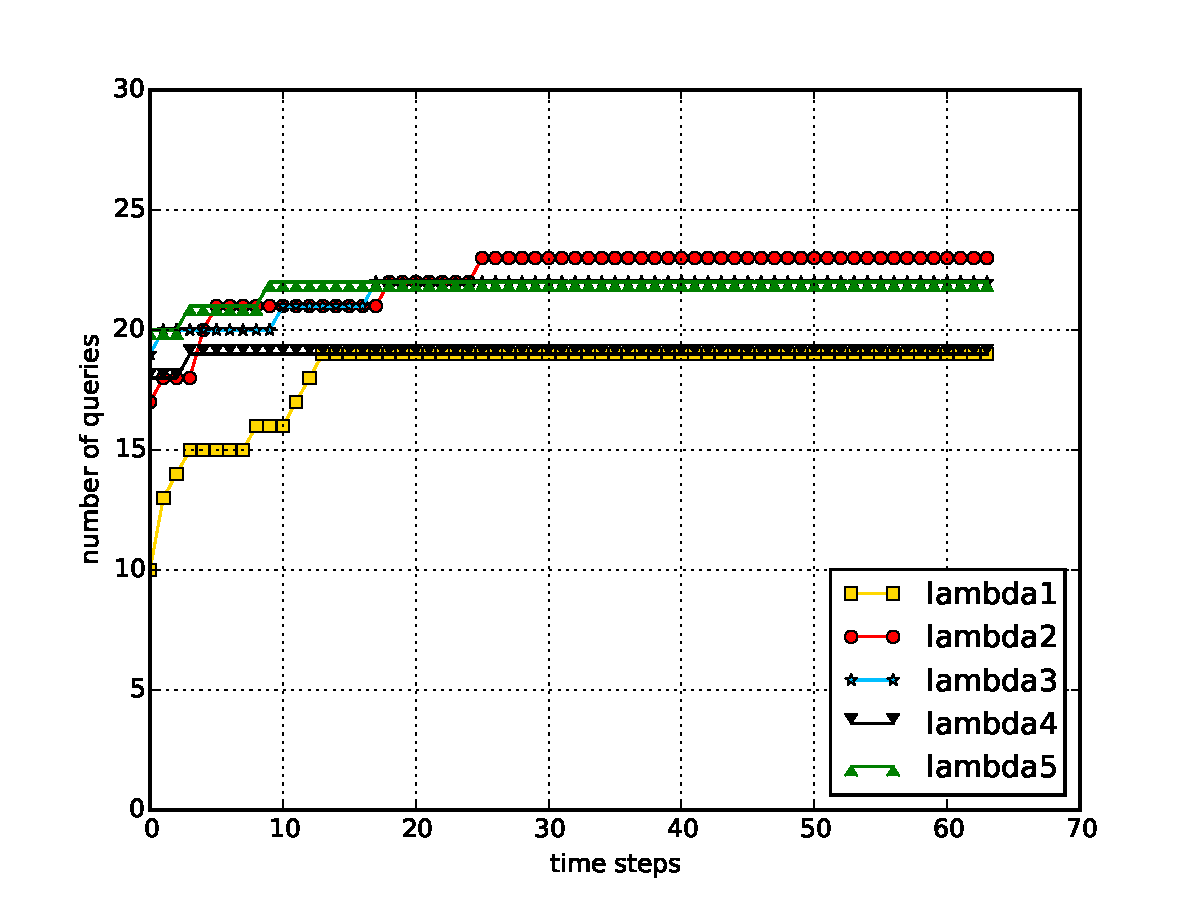
\includegraphics[width=8cm]{graphs/query-complete}
\caption{this figure shows the number of queries proposed to the user during each time step.}
\centering
\end{figure}

\begin{figure}[t]
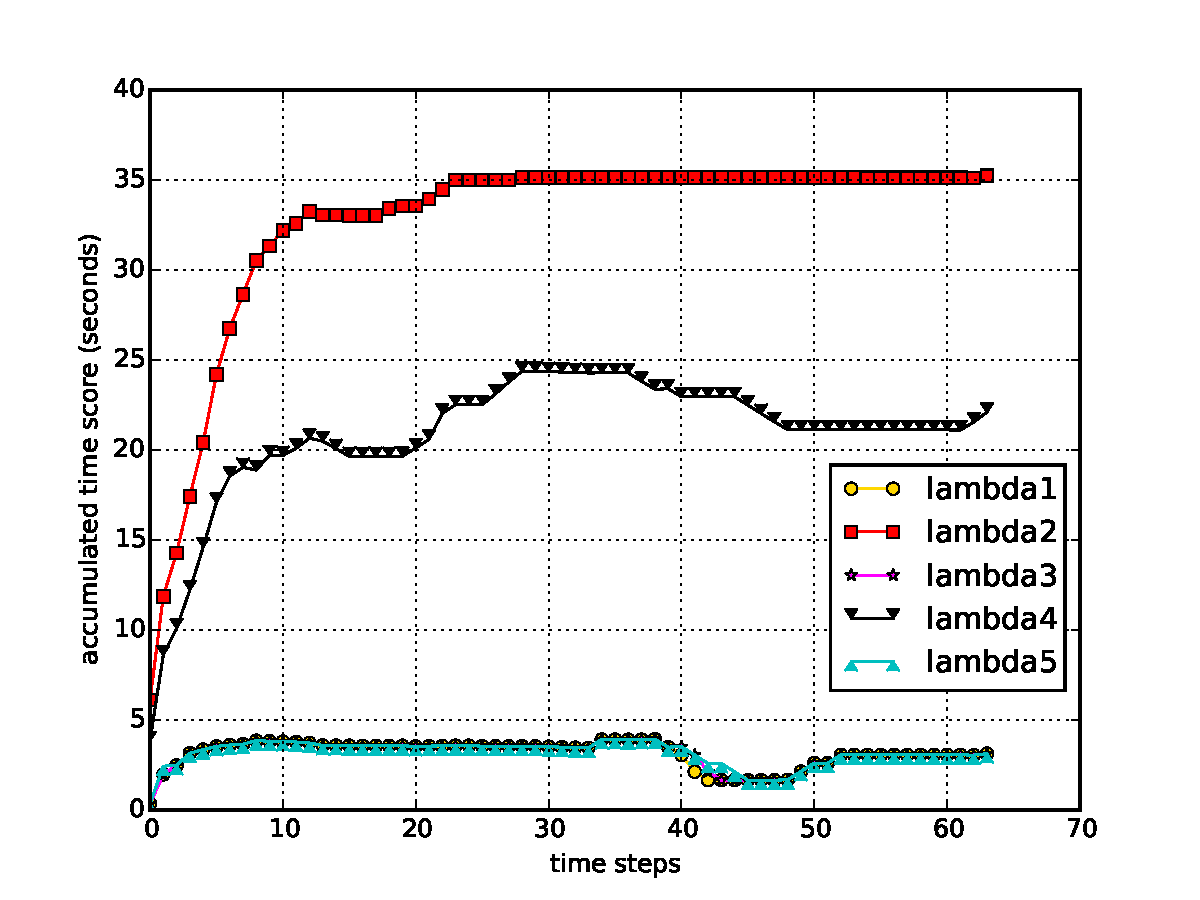
\includegraphics[width=8cm]{graphs/rt_step}
\caption{this figures demonstrates how the accumulated response time increases during each time step. The lambda preferences are as follow:  $\bar{\lambda}_1 =[0.07075913789991828, 0.9292408621000817]$, $\bar{\lambda}_2 = [0.8573741847324399, 0.14262581526756013]$, $\bar{\lambda}_3 = [0.1696287781131175, 0.8303712218868825]$, $\bar{\lambda}_4 = [0.6451844883834318, 0.3548155116165682]$ and $\bar{\lambda}_5 = [0.18190820427369447, 0.8180917957263055]	$}
\centering
\end{figure}

\begin{figure}[t]
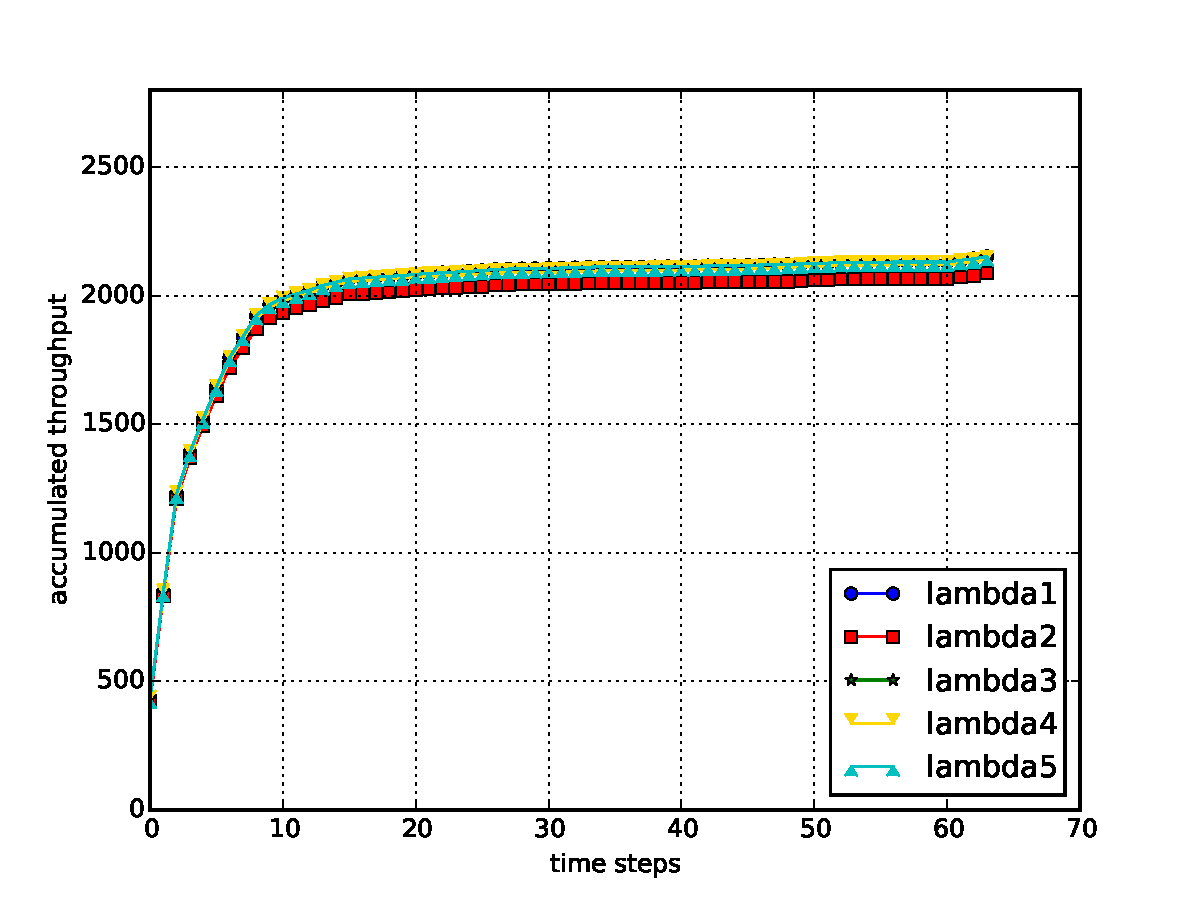
\includegraphics[width=8cm]{graphs/trough_step}
\caption{this figures demonstrates  how the accumulated throughout increases during each time step. The lambda preferences are as follow:  $\bar{\lambda}_1 =[0.07075913789991828, 0.9292408621000817]$, $\bar{\lambda}_2 = [0.8573741847324399, 0.14262581526756013]$, $\bar{\lambda}_3 = [0.1696287781131175, 0.8303712218868825]$, $\bar{\lambda}_4 = [0.6451844883834318, 0.3548155116165682]$ and $\bar{\lambda}_5 = [0.18190820427369447, 0.8180917957263055]	$}
\centering
\end{figure}


We evaluate our methods on a public available dataset containing two parameters for quality of services: response time and throughput. These are the records between $339$ users and $5825$ web services distributed worldwide \cite{10.1109/TSC.2012.34}. The dataset also includes some information about user features, service features such as countries, autonomous systems, IP dresses, latitude and longitude. In the studied data base \cite{10.1109/TSC.2012.34}, users execute various web services in different time slices. Practically, the information are given only for $64$ time steps. 

In this section, we explain first how to model the studied dataset as a VMDP-SC and then we will examine our algorithm on the dataset in two different approaches including the divided dataset based on the users' existed information and  a filtered version of database. 

\subsection{Model DataSet as MOMDP}
The main issue in implementing Algorithm~\ref{algo:ivi} on any database is that how to model the given set as a multi-objective MDP. In the supported dataset \cite{10.1109/TSC.2012.34} there are several text files including wslist.txt, userlist.txt, rtdata.txt and tpdata.txt. Using the wslist.txt, we extract a list of web services and their related abstract services, if a related abstract service exist for the selected web service. In total there are $5825$ web services and $137$ abstract services. The userlist.txt includes the information about $338$ users of different web services. The two other files rt.txt and tp.txt are consist of the data about user execution of web services in $64$ different time steps on response time and throughput respectively. The point is that, they present the related results of $142$ system users. That means at the end, each tested web services with a special user has two parameters for measuring the service quality: response time and throughout. 

According to the extracted information from the database and VMDP-SC definition (see~\ref{def:vmdp-sc}) we have:
\begin{itemize}
\item[-] number of episodes:  $N=64$
\item[-] $137$ number of abstract services 
\item[-] $5825$ number of concrete services (in our case web services)
\item[-]  The transition function and terminal states depends on the proposed model or relation among the abstract services. 
\begin{itemize}
\item[1] For the sequential model (see Fig~\ref{fig:seq-mdp}) the start sate ia an empty state which us connected to the first selected abstract services in the model.  While the terminal state is an empty state for that indicate the the MDP is finite horizon. The probability transitions $P_t(as' | as, sc)$ is $1$ if web service $sc$ for abstract service $as$ is available (according to our database) and abstract service $as'$ is the next state in our selected sequential MDP model for all time steps $t=0 \cdots 63$. 
\item[2] For the parallel model (see Fig~\ref{fig:par-mdp}), the start and terminal states are the empty sates such that the start state has access to the all abstract services and the abstract services are connected to the terminal state based on the possible web services for each one. In this case, $Pt(as'|as, sc)$ is $1$ if $as'$ is the terminal state otherwise it is $0$ for all time step $t = 0, \cdots, 63$. 
\end{itemize}
\item[-] and the $\overline{QoS}_t$ function is build based on the extracted data on web services and their two qualities (response time and throughout).
\end{itemize}

\begin{figure}[t]
\label{fig:seq-mdp}
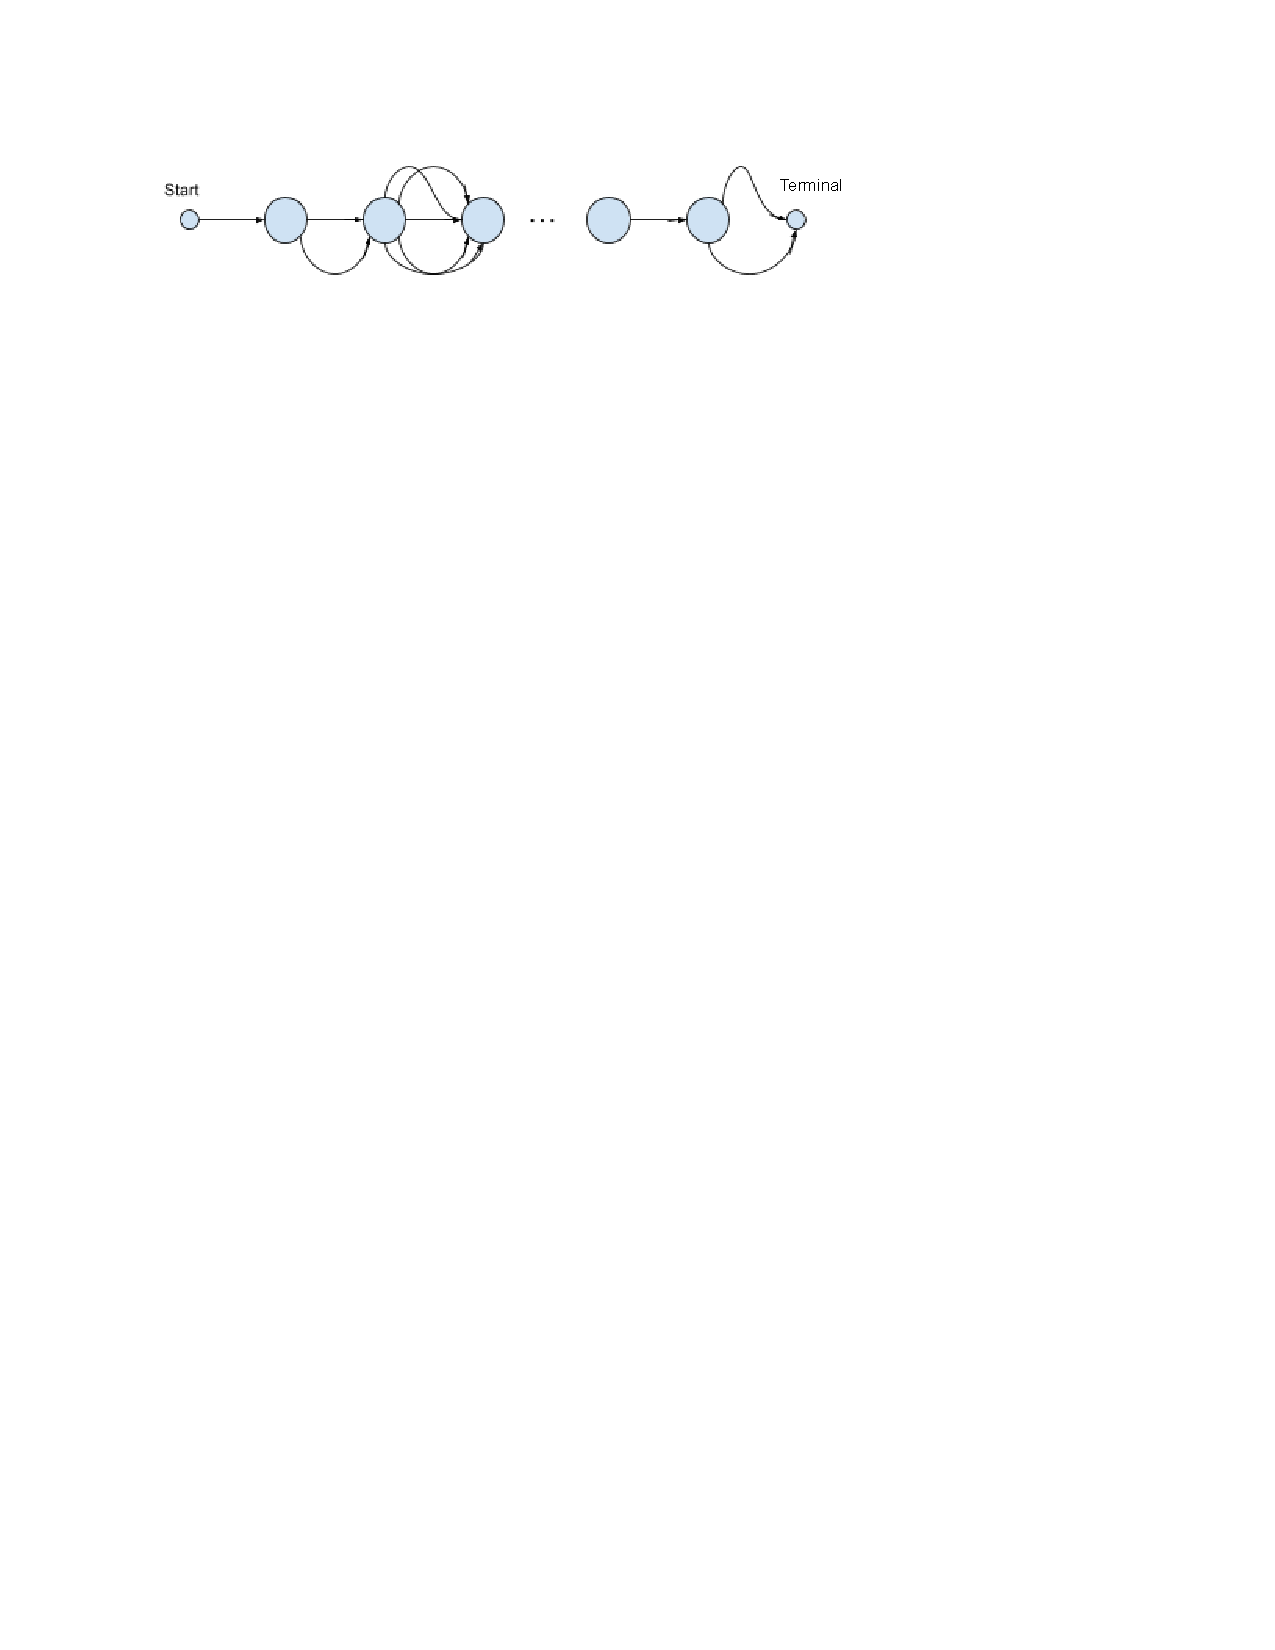
\includegraphics[width=8cm]{graphs/seq-mdp}
\caption{A sequential form of abstract service connection}
\centering
\end{figure}

\begin{figure}[t]
\label{fig:par-mdp}
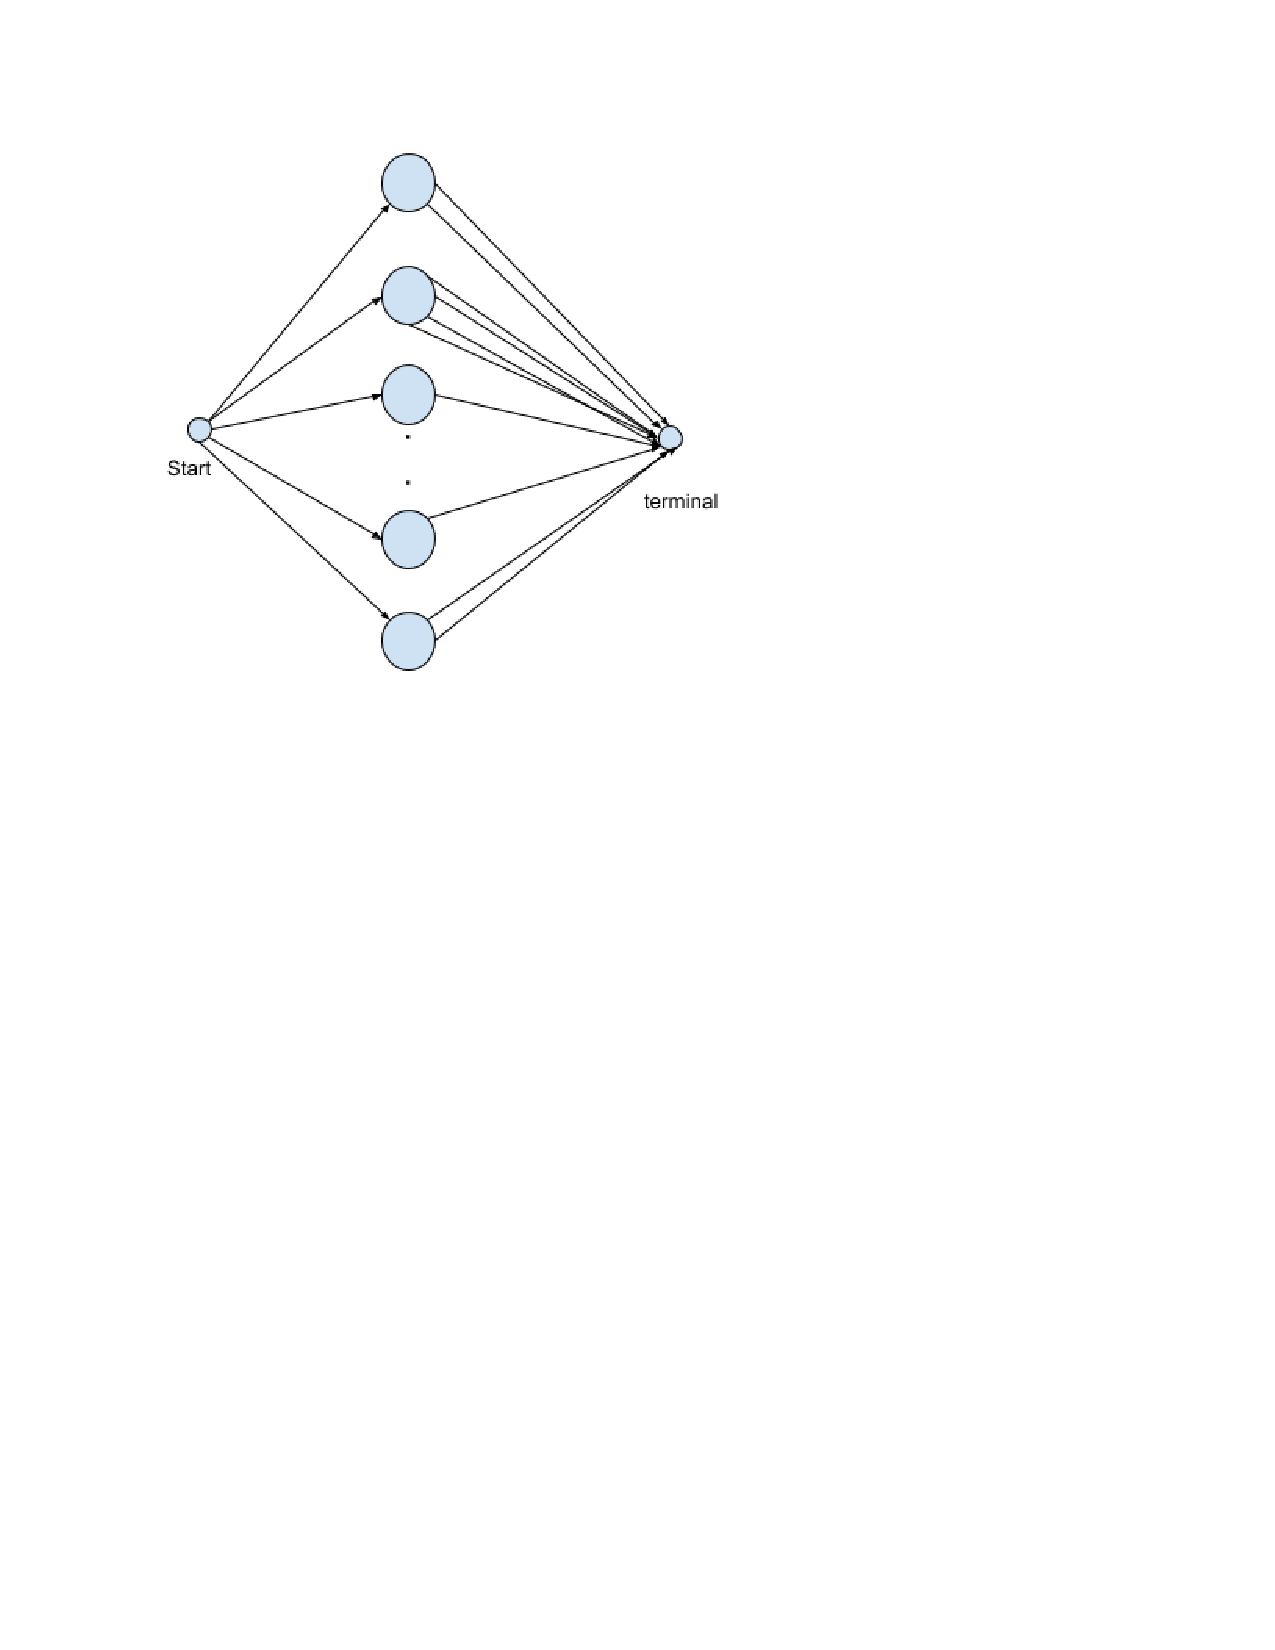
\includegraphics[width=8cm]{graphs/par-mdp}
\caption{A parallel form of abstract service connection}
\centering
\end{figure}

\subsection{Classified Dataset}

\subsection{Filtered Dataset}

Our dataset is a real database generated by observing various users using nonvenomous number of web services. Then, all data inside database are not useful. After extracting all web services and their related abstract services from wslist.tx file, and getting the quality of web services of two files tp.txt and rt.txt, we re recognize that there is no information on some web services related to some abstract services. For this reason, we remove the abstract services without any information on their related web services. 

%\begin{table}[ht]
%\centering
%\resizebox{\columnwidth}{!}{%
%\begin{tabular}{lc|cc||cc||cc||cc||c}
%\hline
% & &  \multicolumn{2}{c||}{User 1} & \multicolumn{2}{c||}{User 2} & \multicolumn{2}{c||}{User 3}  & \multicolumn{2}{c||}{User 4}\\
%\hline
%Services & \shortstack{ \tiny{number} \\ \tiny{of WS}} &IVI& Exact & col3 & col4 & col5 & col6 & col7 & col8\\
%\hline
%AS1659& 1 &2585 & 2585 & 2585 & 2585 & \ra & \ra & \ra & \ra\\
%AS156&2 &4179 & 4179 & 4179 & 4179 & \ra & \ra & \ra & \ra\\
%AS559&2& None & None & None & None & \ra & \ra & \ra & \ra \\
%AS553& 2&1466 & 1466 &\cellcolor{blue!25} 1466 &\cellcolor{blue!25} 1448 & \ra & \ra & \ra & \ra \\
%AS2852& 2&920 & 920 & 920 & 920 & \ra & \ra & \ra & \ra \\
%%\rowcolor{red}
%AS17& 4&\cellcolor{red!25} 4133 & \cellcolor{red!25} 4136 & \cellcolor{blue!25} 4133 &\cellcolor{blue!25} 4136 & \ra & \ra & \ra & \ra \\
%AS7377&5& 3778 & 3778 & 3778 & 3778 & \ra & \ra & \ra & \ra \\
%AS18&1& None & None & None & None & \ra & \ra & \ra & \ra \\
%AS2107&1& 2347 & 2347 & 2347 & 2347 & \ra & \ra & \ra & \ra \\
%AS2900&1& None & None & None & None & \ra & \ra & \ra & \ra \\
%AS224& 9& 2115 & 2115 & 2115 & 2115 & \ra & \ra & \ra & \ra\\
%%\rowcolor{red}
%AS2200&29&\cellcolor{red!25} 1052 &\cellcolor{red!25} 1108 & \cellcolor{blue!25} 1049 & \cellcolor{blue!25} 1108 & \ra & \ra & \ra & \ra \\
%%\rowcolor{red}
%AS25&1& None & None & None & None & \ra & \ra & \ra & \ra \\
%%\rowcolor{red}
%AS5786&3& \cellcolor{red!25} 2213 & \cellcolor{red!25} 2214 &  \cellcolor{blue!25}  2212 & \cellcolor{blue!25}  2214 & \ra & \ra & \ra & \ra \\
%%\rowcolor{red}
%AS680& 44 &\cellcolor{red!25} 1401 & \cellcolor{red!25} 1398 &  \cellcolor{blue!25} 1227 &  \cellcolor{blue!25} 1326 & \ra & \ra & \ra & \ra \\
%AS1930&2 &2204 & 2204 &  \cellcolor{blue!25} 2208 &  \cellcolor{blue!25} 2204 & \ra & \ra & \ra & \ra \\
%AS137&2 &None & None & None & None & \ra & \ra & \ra & \ra \\
%AS239&3& None & None & None & None & \ra & \ra & \ra & \ra \\
%AS131&4& 4060 & 4060 & 4060 & 4060 & \ra & \ra & \ra & \ra \\
%AS237& 6&816 & 816 & 816 & 816 & \ra & \ra & \ra & \ra \\
%AS786& 254&3013 & 3013 & 3013 & 3013 & \ra & \ra & \ra & \ra\\
%AS32& 9& 4388 & 4388 & 4388 & 4388 & \ra & \ra & \ra & \ra  \\
%AS1741&2& 1043 & 1043 & 1043 & 1043 & \ra & \ra & \ra & \ra \\
%AS209&34& 4031 & 4031 & 4031 & 4031 & \ra & \ra & \ra & \ra \\
%AS5723&7& 3832 & 3832 & 3832 & 3832 & \ra & \ra & \ra & \ra  \\
%AS111&1& 4239 & 4239 & 4239 & 4239 & \ra & \ra & \ra & \ra \\
%AS52&3& 4464 & 4464 & 4464 & 4464 & \ra & \ra & \ra & \ra \\
%AS3&2& None & None & None & None & \ra & \ra & \ra & \ra  \\
%AS9&1& None & None & None & None & \ra & \ra & \ra & \ra  \\
%AS8&3& 3668 & 3668 & 3668 & 3668 & \ra & \ra & \ra & \ra  \\
%AS3112&2& None & None & None & None & \ra & \ra & \ra & \ra\\
%AS4538&3& 817 & 817 & 817 & 817 & \ra & \ra & \ra & \ra \\
%AS7132&6& 4209 & 4209 & 4209 & 4209 & \ra & \ra & \ra & \ra \\
%AS19262&19& 3900 & 3900 & 3900 & 3900 & \ra & \ra & \ra & \ra \\
%AS766&11& 2366 & 2366 & 2366 & 2366 & \ra & \ra & \ra & \ra \\
%AS760&4& 91 & 91 & 91 & 91 & \ra & \ra & \ra & \ra \\
%%\rowcolor{red}
%AS73& 5&\cellcolor{red!25} 3911 & \cellcolor{red!25} None &  \cellcolor{blue!25} 3911 & \cellcolor{blue!25} None & \ra & \ra & \ra & \ra \\
%AS20130&2& 3695 & 3695 & 3695 & 3695 & \ra & \ra & \ra & \ra \\
%AS2497&1& 1885 & 1885 & 1885 & 1885 & \ra & \ra & \ra & \ra \\
%%\rowcolor{red}
%AS13041&24& \cellcolor{red!25} 2368 & \cellcolor{red!25} None & \cellcolor{blue!25} 2368 &\cellcolor{blue!25} None & \ra & \ra & \ra & \ra\\
%AS7018&5& 4393 & 4393 & 4393 & 4393 & \ra & \ra & \ra & \ra \\
%AS87&5& 4112 & 4112 & 4112 & 4112 & \ra & \ra & \ra & \ra \\
%\hline
%\end{tabular}
%}
%\end{table}

\begin{figure}[h] % Do not use only [h] in real documents.
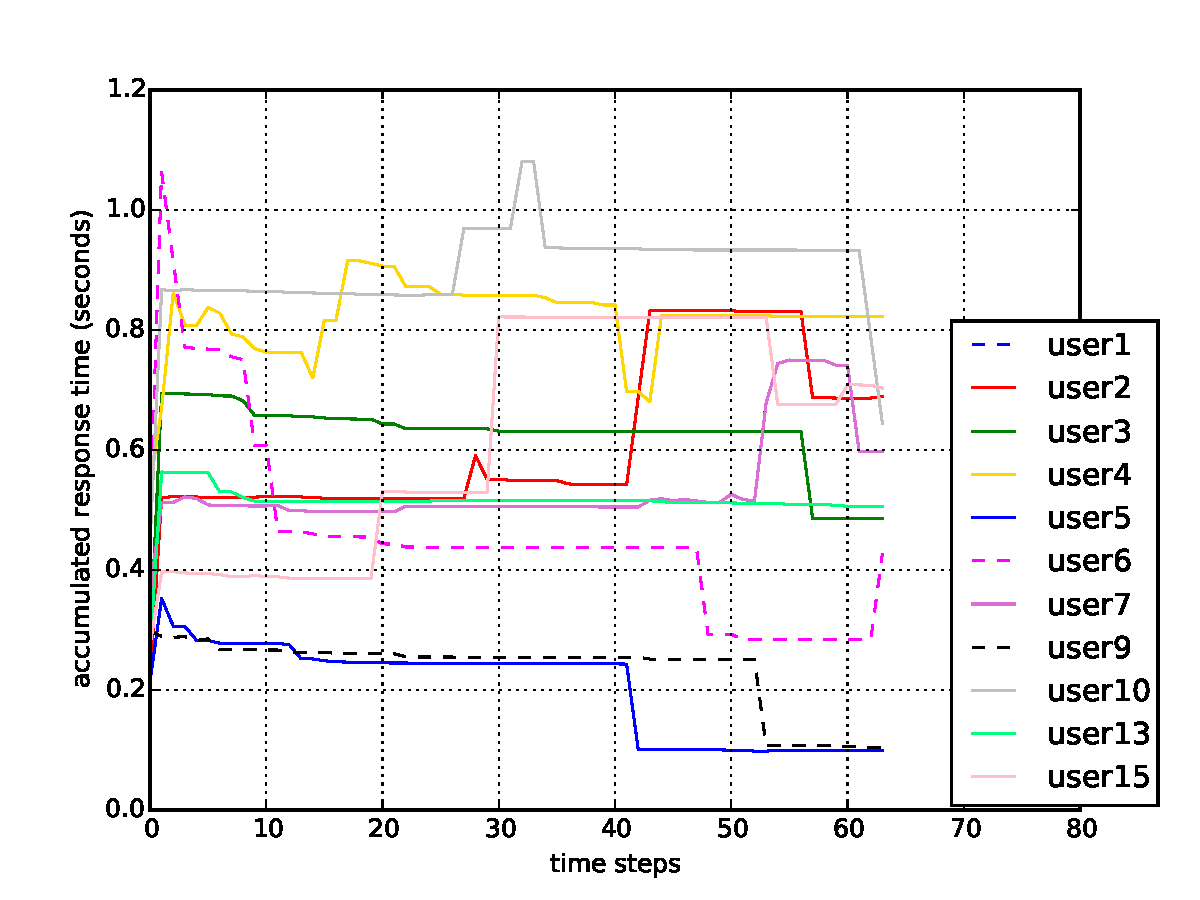
\includegraphics[width=\linewidth]{graphs/rt_step_lambda1}
\caption{ accumulated response time vs time step for several users extracted from the main data base for  $\bar{\lambda}_1 =[0.07075913789991828, 0.9292408621000817]$}
\end{figure}

\begin{figure}[h]
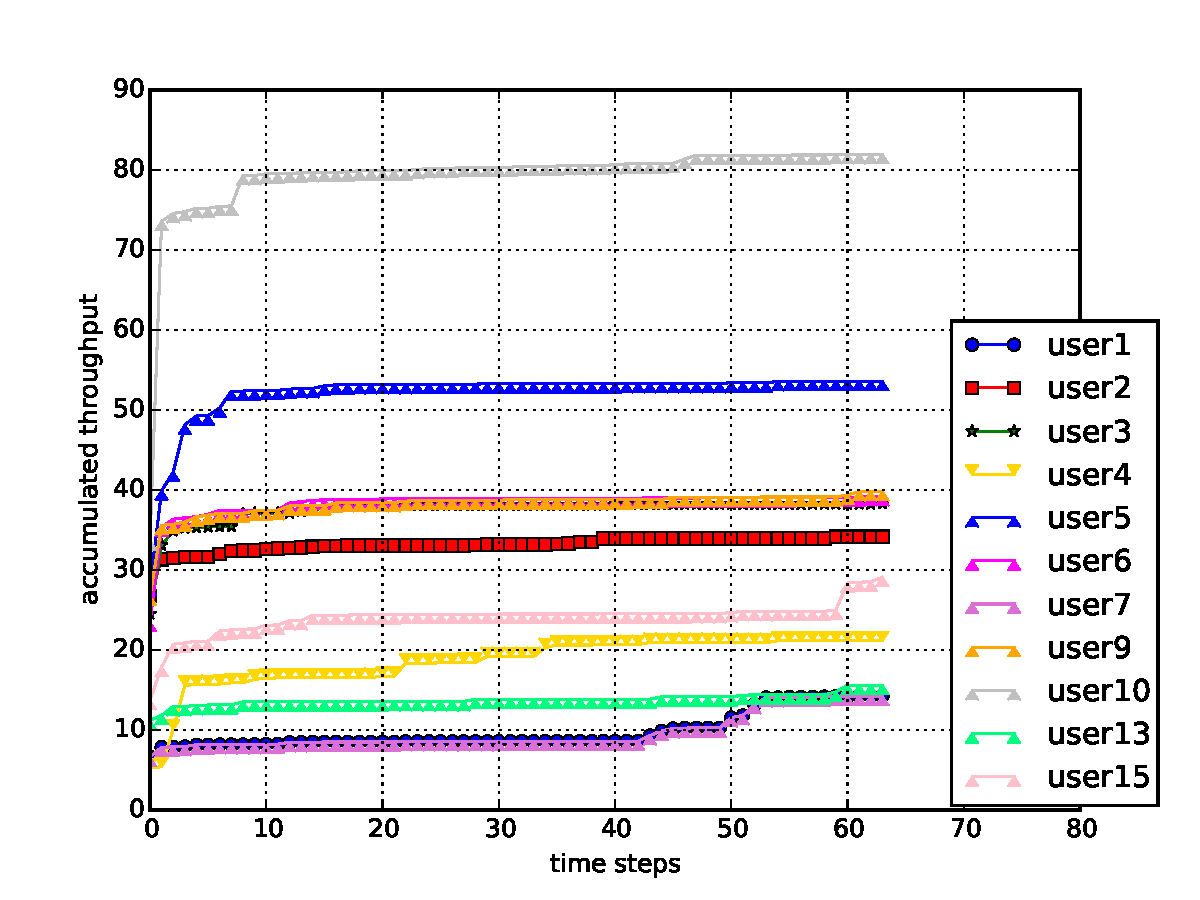
\includegraphics[width=\linewidth]{graphs/trough_step_lambda1}
\caption{accumulated throughout vs time step for several users extracted from the main data base for $\bar{\lambda}_1 =[0.07075913789991828, 0.9292408621000817]$}
\end{figure}

\begin{figure}[h] % Do not use only [h] in real documents.
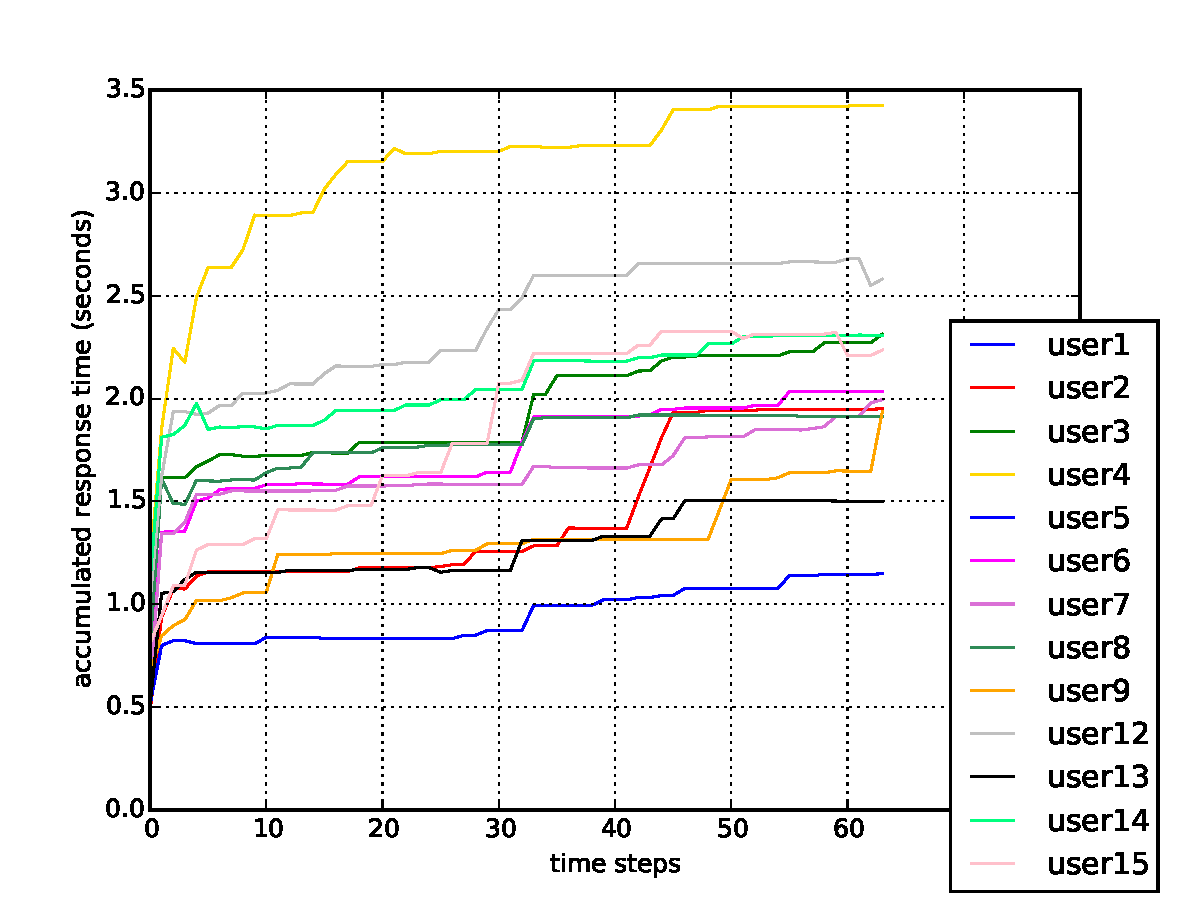
\includegraphics[width=\linewidth]{graphs/rt_step_lambda2}
\caption{ accumulated response time vs time step for several users extracted from the main data base for  $\bar{\lambda}_2 = [0.8573741847324399, 0.14262581526756013]$}
\end{figure}

\begin{figure}[h]
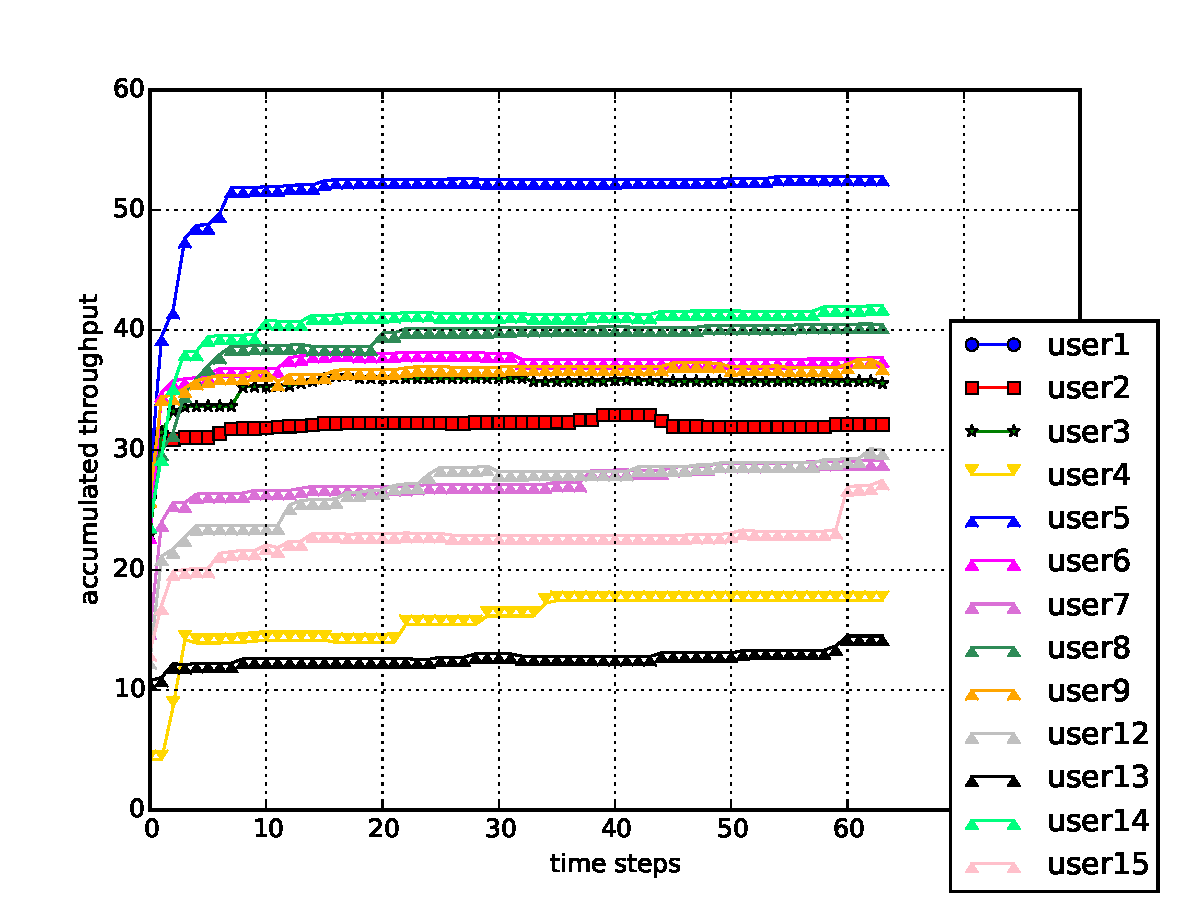
\includegraphics[width=\linewidth]{graphs/trough_step_lambda2}
\caption{accumulated throughout vs time step for several users extracted from the main data base for $\bar{\lambda}_2 = [0.8573741847324399, 0.14262581526756013]$}
\end{figure}

\begin{figure}[h] % Do not use only [h] in real documents.
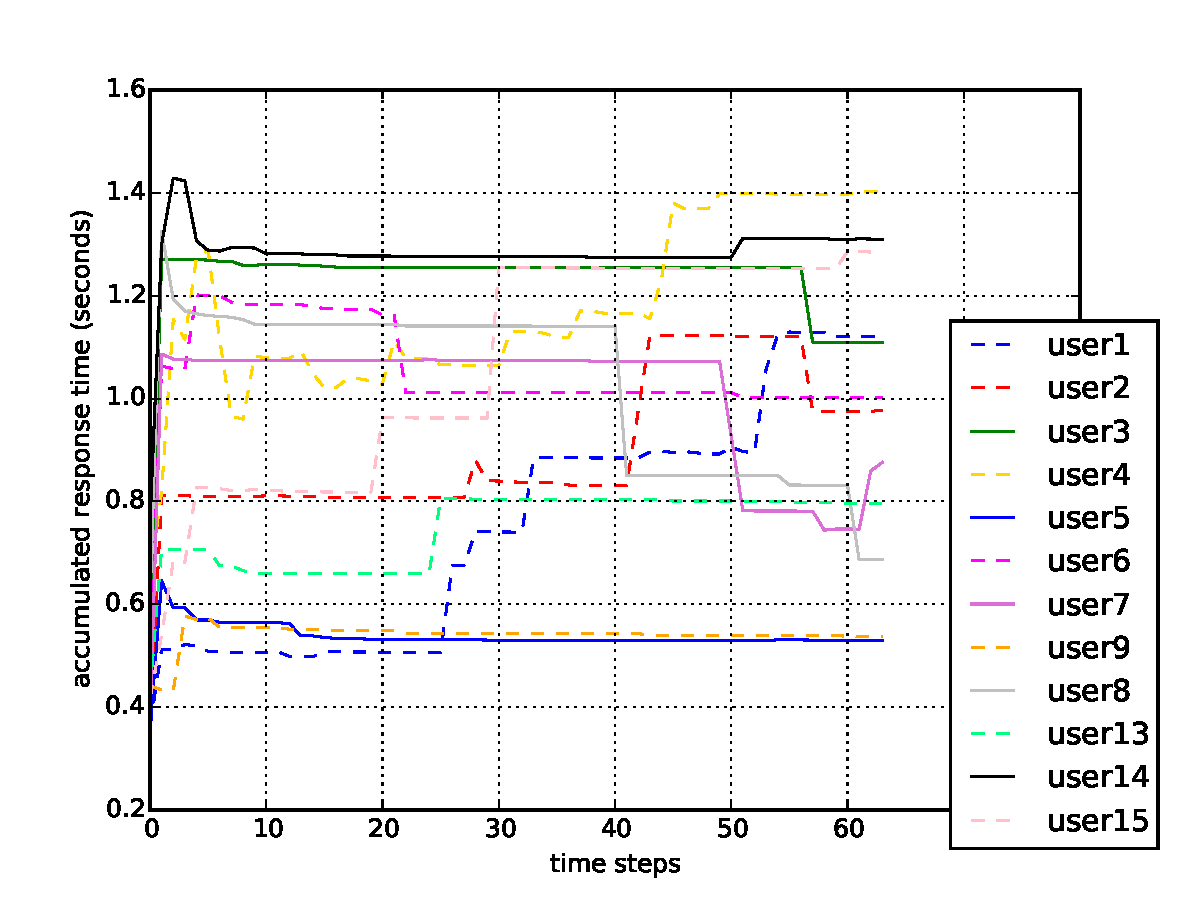
\includegraphics[width=\linewidth]{graphs/rt_step_lambda3}
\caption{ accumulated response time vs time step for several users extracted from the main data base for   $\bar{\lambda}_3 = [0.1696287781131175, 0.8303712218868825]$}
\end{figure}

\begin{figure}[h]
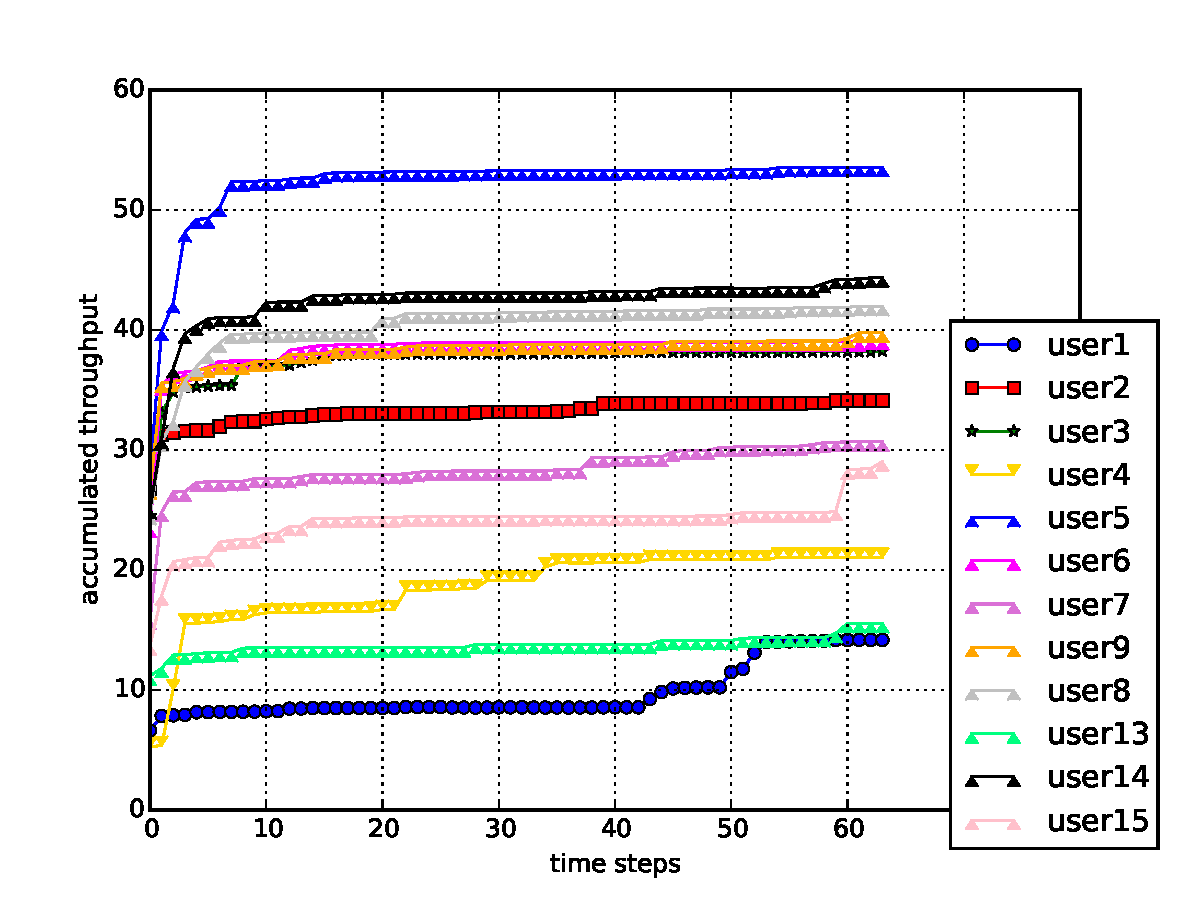
\includegraphics[width=\linewidth]{graphs/trough_step_lambda3}
\caption{accumulated throughout vs time step for several users extracted from the main data base for $\bar{\lambda}_3 = [0.1696287781131175, 0.8303712218868825]$}
\end{figure}

\IEEEpeerreviewmaketitle


% conference papers do not normally have an appendix



% use section* for acknowledgment
\ifCLASSOPTIONcompsoc
  % The Computer Society usually uses the plural form
  
  
  \section*{Acknowledgments}
\else
  % regular IEEE prefers the singular form
  \section*{Acknowledgment}
\fi

The authors would like to thank...


\bibliographystyle{apalike} 
%\bibliographystyle{SIGCHI-Reference-Format}
\bibliography{sample}


% that's all folks
\end{document}


